\documentclass[a4paper,12pt,twoside]{book}

%--------------------------------------------------------------------------
%Packages
%--------------------------------------------------------------------------
\usepackage{amsfonts,amsmath,amssymb}
%\usepackage{amsthm}
\usepackage{xspace}
\usepackage{fancyhdr}
\usepackage{pythonhighlight}

%\usepackage{these}
\usepackage{textcomp} % for degrees : command \textcelsius also \textangle for angles

%\usepackage{epsf}
\usepackage[bookmarks=true,pdftex,colorlinks=true,urlcolor=blue,pdfstartview=FitH]{hyperref}
  \pdfcompresslevel=9
  \hypersetup{
    pdftitle={Practical course reader on control of part},
    pdfauthor={A. de La Fortelle},
    pdfsubject={HDR},
    pdfkeywords={ITS}
  }
\usepackage[pdftex]{graphicx}
\DeclareGraphicsExtensions{.jpg,.mps,.pdf,.png} % Formats d'images
\graphicspath{{Figures/}} % Chemin vers les figures



%----------begin commands----------
\newcommand{\ud}{\mathrm d} %COMMENT: for infinitesimal dx = \ud x and dy = \ud y TODO: DO YOURSELF all replacement
\renewcommand\theequation{\arabic{equation}}
\renewcommand{\figurename}{Fig.}
\newcommand{\subgroup}[2]{\medskip \emph{Prepared by subgroup #1 (#2)}\medskip}
%----------end commands----------


%--------------------------------------------------------------------------
%Document
%--------------------------------------------------------------------------
\begin{document}
\frontmatter
\thispagestyle{empty}
\topmargin -5mm
%\textheight 25cm
%\enlargethispage{4cm}
\headsep 0cm
\font\tensmc=cmcsc10 scaled 1200
%\font\grand=cmbx12 scaled 3000
\font\grand=cmbx12 scaled 1600
\font\moyen=cmbx12 scaled 1200

\noindent
Version: \today
%version finale du \today.


\vskip 1cm

%\centerline{.}
%\centerline{\rule{\textwidth}{2mm}}
\begin{center}
{\grand  Practical Course Reader

\bigskip for Control of distributed systems}

\vspace{2cm}
{        made at the}\bigskip

{\moyen  University of California at Berkeley} \medskip

\vskip 0.8 cm
{\tensmc by \moyen Arnaud de LA FORTELLE}
\vskip 0.8 cm
{\moyen  visiting professor from MINES ParisTech} \medskip


%\vskip .4cm
\vfill
\centerline{\hbox to 3cm{\leaders\hrule\hfil}}
\vskip .3cm
\smallskip

{\moyen for the course CE-C291F --- EE-C291 --- ME-C236}

\smallskip
\smallskip
\centerline{\hbox to 3cm{\leaders\hrule\hfil}}
\end{center}
\vskip 0.5cm plus 0.6cm



\vfill
With the help of:
\begin{center}
\begin{tabular}{lll}
%MM. & {\bf Bradley Cage} & student\\
& {\bf Bradley Cage} & student\\
& {\bf Hongbei Chen } & student\\
& {\bf Yue Hu } & student \\
& {\bf Carlin Liao} & student\\
& {\bf Xin Peng} & student\\
& {\bf Robert Ruigrok } & student\\
& {\bf Lin Yang} & student\\
& {\bf Qingan Zhao } & student\\
& {\bf Ruitong Zhu } & student
 %\phantom
\end{tabular}
\end{center}

%\centerline{--\ 2000\ --}

\newpage

\pagestyle{fancy}
\addtolength{\headsep}{\marginparsep}
\addtolength{\headheight}{\baselineskip}
%\addtolength{\headwidth}{\marginparsep}
%\addtolength{\headwidth}{\marginparwidth}
%\renewcommand{\chaptermark}[1]{\markboth{#1}{#1}} % remember chapter title
%\renewcommand{\sectionmark}[1]{\markright{\thesection\ #1}}
\renewcommand{\chaptermark}[1]{\markboth{\thepart~~Ch.~\thechapter\ \ #1}{#1}}
\renewcommand{\sectionmark}[1]{\markright{\thesection\ #1}}
\fancyhf{}
%\fancyhead[LE,RO]{\bfseries\thepage}
\fancyhead[LE,RO]{\thepage}
\fancyhead[LO]{\small \sc \rightmark}
\fancyhead[RE]{\small \sc \leftmark}
\fancypagestyle{plain}{
\fancyhead{}
\renewcommand{\headrulewidth}{0pt}
}




%\href{Table of contents}{}
\tableofcontents
\addcontentsline{toc}{chapter}{Table of Contents}

%\listoffigures

\mainmatter

\thispagestyle{empty}
%----------------------------------------------------------------------
\chapter{Introduction}
\label{introduction.chap}
%----------------------------------------------------------------------

\section{Objectives}
%----------------------------------------------------------------------

This practical course reader aims at giving good advice to students realizing a project. Starting with the theoretical knowledge contained in the reader of Prof. Alexandre Bayen, students have to realize a project based on a distributed parameter system that they should:
\begin{enumerate}
	\item describe
	\item model
	\item explain
\end{enumerate}
The first part is a descriptive (i.e. qualitative) description of the system to be studied, its interest and the goal of the study. The second part is an elaboration, under simplifications, of a quantitative model (meaning here some kind of Partial Differential Equation and some control or optimization). The third part is an analysis of this model, either by solving the equations, by simulation or by a combination of both, using the tools learned during the course. It should lead to a better understanding of how the system works and how it can be optimized or controlled to fulfill the goals set in the description.

Therefore this practical course reader shows examples of modeling and various analysis methods that can support the creativity of the students realizing a project.

\section{System description}\label{description.sec}
%----------------------------------------------------------------------
A system is, according to Cambridge dictionary ``a set of connected things or devices that operate together''. There is no recipe to describe a system. However, it is often useful, instead of having an \emph{analytical} description (i.e. tear the system into pieces), to have a \emph{synthetic} one (i.e. seeking for a global view). Without any generalization, again, one can look after the following 4 views of a system:
\begin{enumerate}
	\item objective
	\item environment
	\item actions
	\item transformations
\end{enumerate}
One can very arguably contest these words, but remember they are only guidelines. In most systems, since they are man-made, there is a goal. This \emph{objective} is important to describe since it contains the meaning: what is it for? Note this is quite often the opposite of the analytical view: how does it work? However, in our case, this goal contains the information about the \emph{objective function} for optimization or for control. The \emph{environment} dictates what the system has to do: a system is never isolated and its goal is often closely related to its environment. At least, the \emph{actions} a system perform are partially internal and partially external, so that taking into account the environment allow understanding of disturbances but also the objective. Since a system is usually complex, it may evolve (i.e. experience \emph{transformations}) according to actions and in line with the objective. One can also think of transformation as internal states of a finite automaton.

In any case, a description is intended at telling the whole story to other people and this is why it is highly recommended to use only words, no formula, but drawings can well replace a thousand words.

\section{System modeling}
%----------------------------------------------------------------------
While a system description is intended to be purely qualitative, modeling aims at estimating some quantities. Very clearly, the choice of the quantities is decisive. Important quantities can be derived from the system description, such as the objective function (what to maximize or minimize?), the transformations (internal states) or environment variables.

There are many ways to measure quantities, e.g. numbers of vehicles in a microscopic view may be equivalent to measuring densities of vehicle at a macroscopic scale. Unfortunately there is no algorithm to produce significant model and this is a knowledge that needs practice. However, in our present case, namely partial differential equations modeling, there is very often a kind of scaling that is necessary in order to produce continuous-space and continuous time variables. Since this reader aims at being practical, the reader is referred to Chapter~\ref{modeling.chap} for modeling examples.

One can (too?) quickly summarize some usual quantities of interest:
\begin{itemize}
	\item macroscopic quantities (temperature, density, deformation...);
	\item variables (state space, time...) and parameters including the control;
	\item optimization criteria;
	\item invariant quantities (mass, energy, momentum...) and constraints;
	\item initial and boundary conditions.
\end{itemize}


\section{System explanation}
%----------------------------------------------------------------------
What is called here explanation has been also called ``solution'' during the course. It consists mainly in studying the model under various views and to produce new knowledge. This usually implies simulations, analytical analysis, optimization and visualization; all previous methods can be compared or combined in order to give more insight of the model.

\subsection{Analysis}\label{analysis.sec}
Analysis is important for the concepts it carries. We have learned a few methods to exactly solve or to transform the PDEs:
\begin{enumerate}
	\item Dimensional analysis allow to build interesting quantities that should remain constant;
	\item Product-form solutions leads to decomposition of solutions (often in the type of Fourrier transform) with knowledge of the modes and their frequencies (spatial and temporal).
	\item the method of characteristics is a powerful methods to build solutions, even discontinuous like shockwaves in LWR equations. The characteristic curves are interesting features.
\end{enumerate}
In the present course, students should perform some initial analytical analysis, even if it does not lead to a complete solution, in order to exhibits interesting quantities as mentioned above. These quantities should be used as guidelines as far as possible for further study.

\subsection{Simulation}\label{simulation.sec}
Simulation is interesting for all the data it brings. However there are many ways to simulate a system. At least we can mention:
\begin{itemize}
	\item Microscopic simulation --- often agent-based --- where a lot of microscopic entities evolves with their dynamics; This method is relevant when the PDE is a macroscopic view of the system, i.e. when it is derived from a scaling;
	\item Finite differences schemes, that is often a direct implementation of the dynamics underlying the PDE (differences apply on a discretization of space and time);
	\item Finite elements is usually associated to computation of eigenvalues and eigenvectors, i.e. to product-form solutions and the computation of modes; in this case, discretization is made through a projection of the functions onto a finite (functional) basis.
\end{itemize}
In this course, students have to produce simulations. The goal is to exploit the data to visualize the system evolution (see also Section~\ref{visualization.sec}) and get a better understanding. One of the main problem of simulation is to have a clear idea of the quantities to be displayed, be it statistics, metrics or functions. This is why a good prior analysis (see also Section~\ref{analysis.sec}) is a good idea. A must in simulation is to compare quantities computed from the output of the simulation with similar quantities computed from theoretical analysis: e.g. number of vehicles per km in micro-simulation with densities in LWR equations.


\subsection{Optimization or control}\label{optimization.sec}
The goal of this course is to learn how a system can be controlled or optimized. This requires to have a good description of the system in order to have clear ideas of what is to be optimized or controlled. Usually, the design of the control is free and this is where students can be creative.

There is a very common distinction between 2 close concepts: planning and control. In most real systems, the planning phase is responsible for building suitable a path, according to the dynamics of the system and to the environment; then, a control loop ensures the systems follows this path by using actuators (the controls) and taking care of disturbances (in sensors and in actuators). Planning is open-loop, usually with a simple model (deterministic...) but with a complex cost function that expresses the desirable behavior. Control is closed-loop, designed to be robust, taking into account noises and disturbances, with a simple cost function: follow the plan.

Techniques are very diverse and really depend on the system and the kind of control. Examples are given in Chapter~\ref{control.chap}.

\subsection{Visualization}\label{visualization.sec}
The visualization aspect of a study may be the most important yet the most challenging. Indeed, a drawing is extremely instructive, provided it is well explained. But the beauty can be misleading and the students have to take great care of the quantities they illustrate: What should be seen in the drawing? What does it tell us? Does it compare well with existing knowledge or not?

Therefore it is advised to start quickly (very early with simulation data) to try to see something and to continuously improve the visualization aspect. It is important for explaining the results as well as for enhancing the students' own understanding (and debugging the codes, very often).

\thispagestyle{empty}
%----------------------------------------------------------------------
\chapter{Modeling}
\label{modeling.chap}
%----------------------------------------------------------------------

\section{Objectives}
%----------------------------------------------------------------------

The modeling of a system starts with a good description (see Section~\ref{description.sec}). Very often, the system can is made of numerous elements (e.g. cars, particles...) or can be decomposed into small chunks (string, heated body...). In this course we want to obtain PDEs: this means that the dynamics is local. Small elements influence only their neighbors through quantities that are very important: tension and curvature for a string, density and flow for traffic... In order to obtain PDEs, it is often necessary to assume such quantities are slowly varying and that one can \emph{scale} the system. Moreover, one should keep only a very limited number of quantities and simplifying assumptions are key to that objective (neglect gravity, torsion, viscosity...). Finally, an equation (even after scaling) is always obtain as limit of another equation: it is important to explain which principles (physical or other) lead to these equations, be it a conservation equation or dynamical equations.

Now, a model is not complete with only a PDE: initial and boundary conditions must be explicit, the control parameter (or the space of choice) must be given as well as the optimization criteria. The following examples illustrate this method. 

\section{Derivation of partial differential equations}
%----------------------------------------------------------------------
This section shows how one can describe some simple systems and derive from physical principles the PDEs modeling their behavior.

\subsection{2D wave equation}
% ***********************************************************************************
% Pure LaTeX part to be inserted in a document (be careful of depencies of packages & commands
% Prepared by XXX and YYY under the supervision of Arnaud de La Fortelle
% Fall 2017
% 2D wave propagation subsection of the modeling part
% ***********************************************************************************

\subgroup{1}{Bradley Cage and Lin Yang

\paragraph{Description}
\begin{figure}[htb]
	\centering
	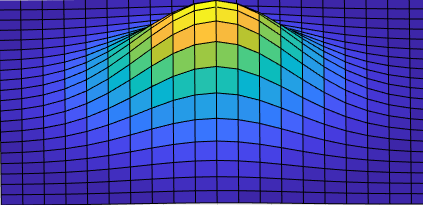
\includegraphics[width=10cm]{Figures/2D_waves_system.png}       
	\caption{The membrane system }
	\label{2D_waves_system.fig}
\end{figure}

Our system is comprised of a flexible membrane stretched to some shape, with all of its edges fixed in place. The desired goal is to understand the vertical position of the various points on the membrane over time. The membrane in this system has vertical deflections which are small compared to its overall size, and deflections happen only in the vertical direction.

This 2D system is a continuation of the 1D wave equation, and is a natural precursor to the 3D wave case. 


\paragraph{Model}
Assumptions:
\begin{itemize}
	\item Membrane has uniform planar density $\rho$
    \item The tension per unit length, $F_t$, caused by stretching the membrane is the same at all points and in all directions and does not change during the motion
    \item Vertical position is given by some function $u(x,y,t)$
\end{itemize}
\begin{figure}[htb]
	\centering
	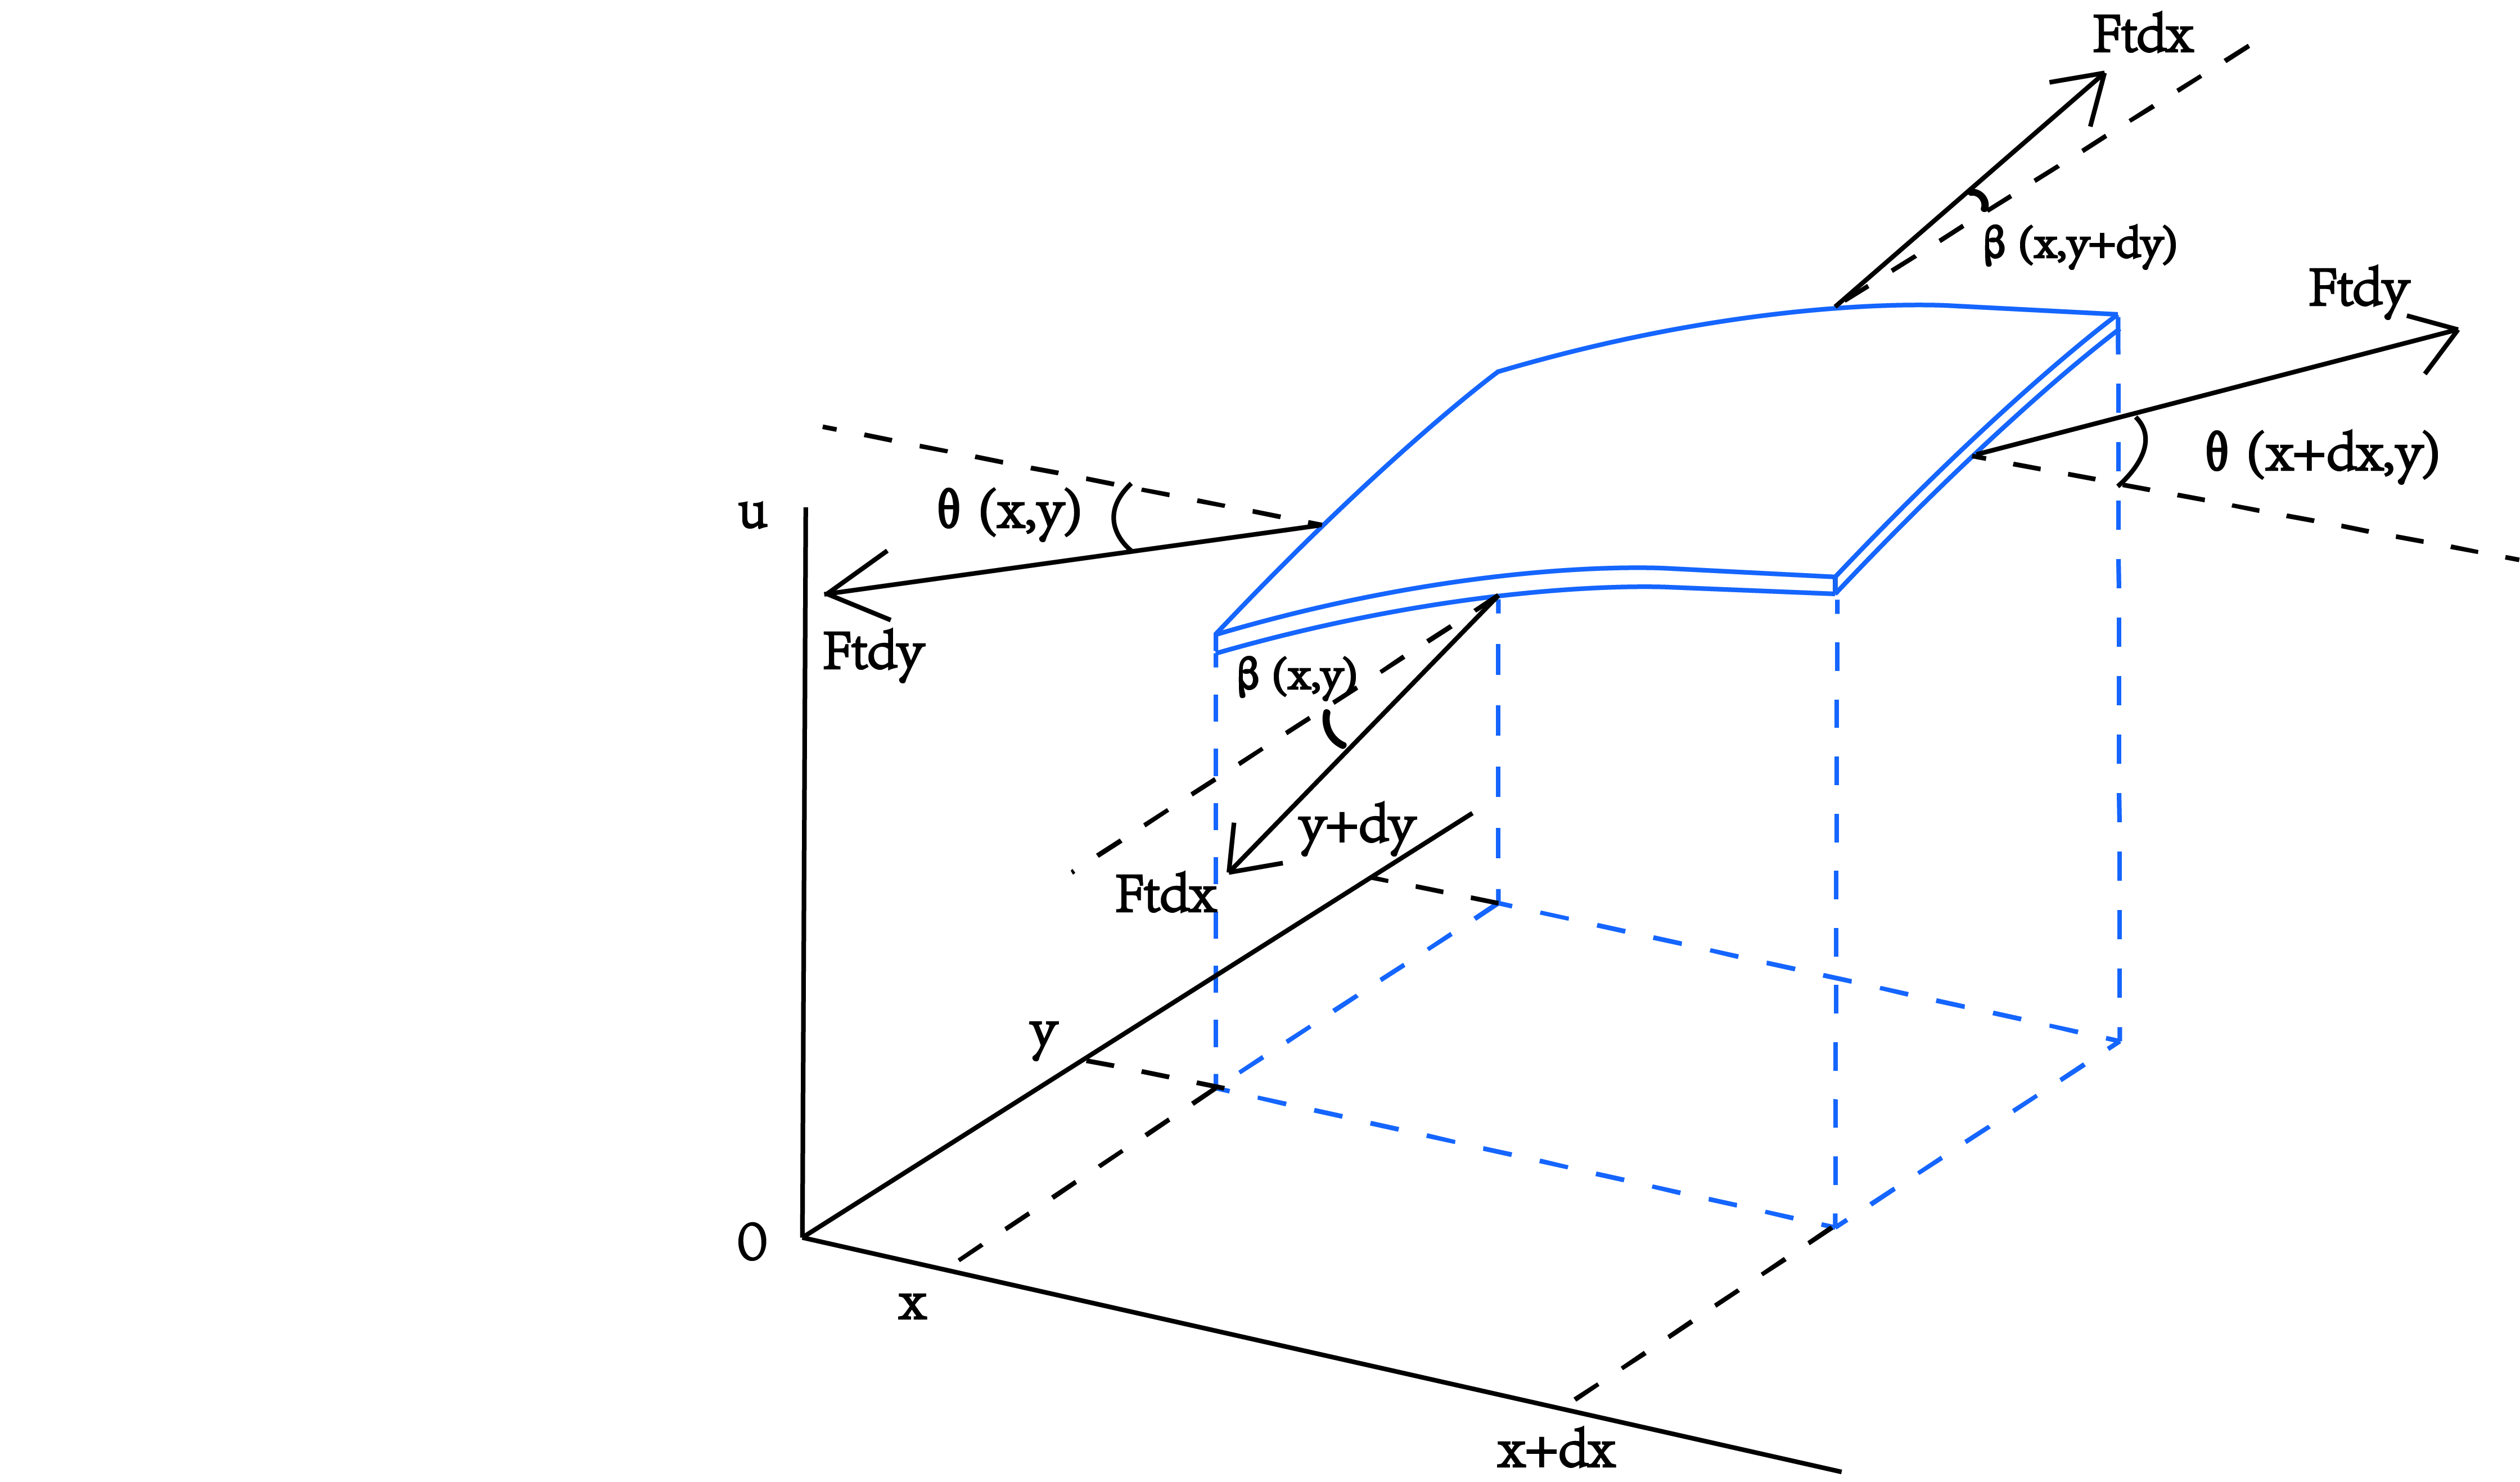
\includegraphics[width=15cm]{Figures/2D_waves_model.png}       
	\caption{The force analysis of a small section of the membrane system }
	\label{2D_waves_model.fig}
\end{figure}
We begin from basic principles.

$$\Sigma F = m\vec{a}$$

\noindent Taking some small section of the membrane $\ud x$ by $\ud y$, we can replace mass and acceleration and since we know density and that $\vec{a}$ is the second derivative of position with respect to time, thus enabling us to rewrite the equation.

\begin{equation}
\label{no_balance}
\Sigma F = \rho \ud x\ud y \frac{\partial^2u}{\partial t^2}
\end{equation}

\noindent Performing a force balance on the section of membrane in the x and y directions gives us tensions at each on each side, then resolved to their vertical components. Remember that since tension is constant per unit length, we must multiply the force acting on each side by the length of that side. Thus, the force acting on this balance lets us rewrite $\Sigma F$ (that is we only consider vertical forces, forces acting in the $x-u$ and $y-u$ planes): 

$$\Sigma F = F_x + F_y$$

$$F_x = F_t\ud y\Big[\sin\big( \theta (x+\ud x,y,t) \big) - \sin \big((\theta (x,y,t)\big)\Big]$$
$$F_y = F_t\ud x\Big[\sin\big( \beta (x,y+\ud y,t) \big) - \sin \big((\beta (x,y,t)\big)\Big]$$

\noindent We can confidently use the small angle approximation $\sin$ in the x direction

$$ \sin(\theta) \approx \tan(\theta) = \frac{\partial u}{\partial x} = u_x$$

\noindent and likewise in the y direction 

$$ \sin(\beta) \approx \tan(\beta) = \frac{\partial u}{\partial y} = u_y$$

\noindent to get our equations into the form

$$F_x = F_t\u dy\Big[u_x(x+\ud x,y,t) - u_x(x,y,t)\Big]$$
$$F_y = F_t\u dx\Big[u_y(x,y+\ud y,t) - u_y(x,y,t)\Big]$$

\noindent From there we can sum these forces and plug them back in to equation \ref{no_balance}

$$\rho \ud x\ud y \frac{\partial^2u}{\partial t^2} = F_t\bigg[dy\Big[u_x(x+\ud x,y,t) - u_x(x,y,t)\Big]+dx\Big[u_y(x,y+\ud y,t) - u_y(x,y,t)\Big] \bigg]$$

\noindent We then divide by $\ud x$ and $\ud y$ and take the limit as $\ud x,\ud y \to 0$:

$$\rho\frac{\partial^2u}{\partial t^2} = \lim_{\ud x,\ud y\to 0} F_t \bigg[ \frac{u_x(x+\ud x,y,t) - u_x(x,y,t)}{\ud x} + \frac{u_y(x,y+\ud y,t) - u_y(x,y,t)}{\ud y} \bigg]$$

\noindent We recognize that we now have derivatives in the form of difference quotients, and can take the partial derivative of each one (since $u$ is a function of multiple variables)

\begin{equation}
\rho \frac{\partial^2u}{\partial t^2} = F_t\bigg[\frac{\partial}{\partial x}u_x + \frac{\partial}{\partial y}u_y \bigg] = F_t\bigg[\frac{\partial^2 u}{\partial x^2} + \frac{\partial^2 u}{\partial y^2}\bigg]
\end{equation}

\noindent Dividing over the uniform  tension, we reach our final form.

\begin{equation}
\frac{\rho}{F_t}\frac{\partial^2u}{\partial t^2} = \frac{\partial^2 u}{\partial x^2} + \frac{\partial^2 u}{\partial y^2}
\end{equation}

\noindent We can adhere to standard conventions and write our final 2D wave equation as 


\begin{align}
a^2 \frac{\partial^2u}{\partial t^2} &= \frac{\partial^2 u}{\partial x^2} + \frac{\partial^2 u}{\partial y^2} & a &= \sqrt{\frac{\rho}{F_t}}
\label{final_eq}
\end{align}

\noindent Equation \ref{final_eq} is also commonly written using the Laplace operator:

\begin{equation}
a^2 \frac{\partial^2u}{\partial t^2} = \nabla^2 u
\end{equation}
\noindent Initial condition:
\begin{itemize}
	\item When t=0, the vertical position all over the membrane is 0, i.e., $u(x,y,0)=0$.
\end{itemize}
\begin{figure}[htb]
	\centering
	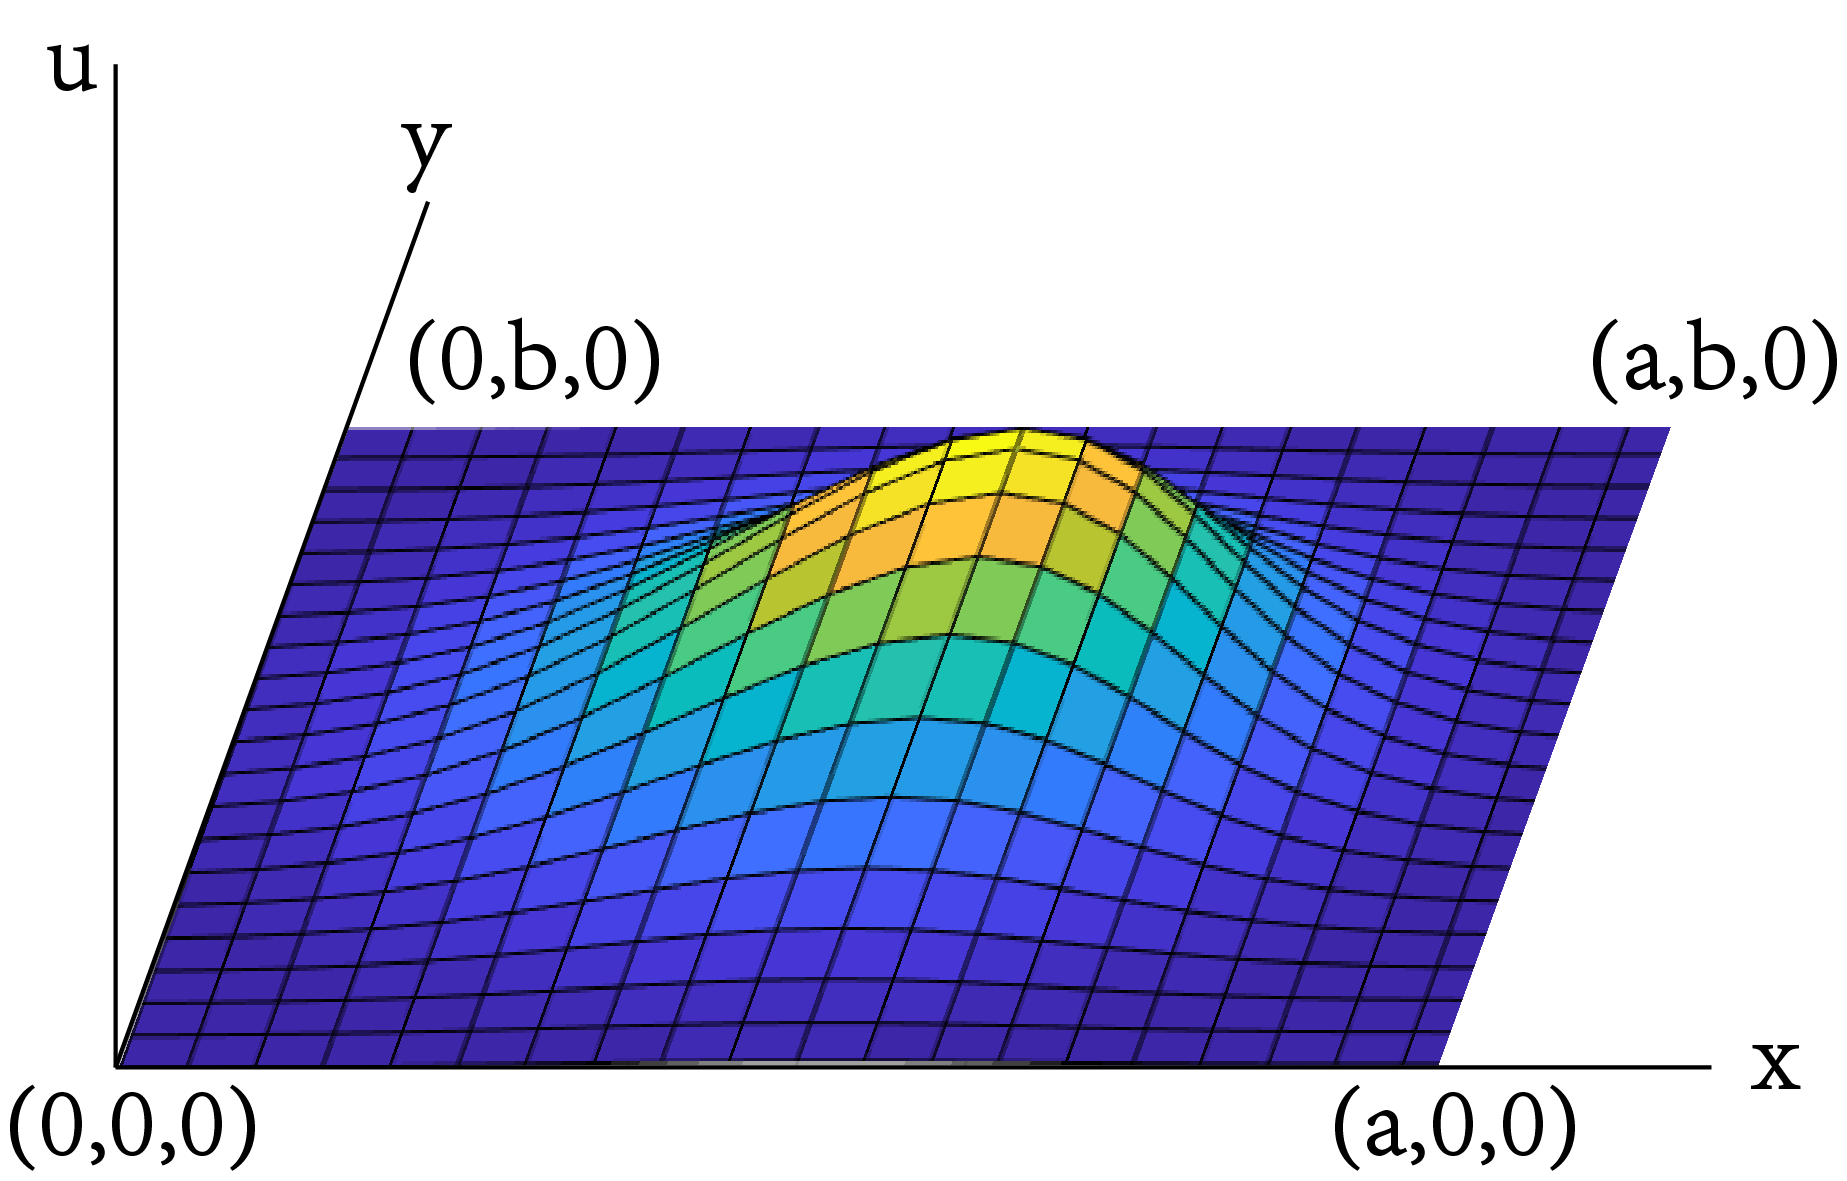
\includegraphics[width=10cm]{Figures/2D_waves_boundary_conditions.png}       
	\caption{The membrane system's boundaries}
	\label{2D_waves_boundary_conditions.fig}
\end{figure}
Boundary condition:
\begin{itemize}
	\item The vertical positions of the 4 edges of the membrane remain 0 all the time, i.e., $u(x,0,t)=0$, $u(0,y,t)=0$, $u(a,y,t)=0$, $u(x,b,t)=0$.
\end{itemize}
\noindent Some hints for the control and the cost function of the 2D wave equation:
\begin{itemize}
	\item Control: Maintain the highest vertical deflection of the membrane to be some constant height H   
    \item The cost function then could be finding the smallest force exerted on the membrane to maintain the highest height H in the membrane system
    
\end{itemize}

\subsection{2D heat diffusion}
% ***********************************************************************************
% Pure LaTeX part to be inserted in a document (be careful of depencies of packages & commands)
% Prepared by Qingan Zhao and Ruitong Zhu under the supervision of Arnaud de La Fortelle
% Fall 2017
% 2D heat diffusion subsection of the modeling part
% ***********************************************************************************

\subgroup{2}{Qingan Zhao and Ruitong Zhu}

\paragraph{Description}
The aim of this part is to describe and model a PDE that describes temperature dynamics in a two-dimensional body via heat conduction.
Basically, heat conduction is the exchange of heat from regions of higher temperatures into regions with lower temperatures, which varies in the transfer rate for different materials.

Consider a thin flat body with a constant thickness $h$ and uniform density $\rho'$. Assume that the faces of the thin body are in perfect insulation, which means there is no heat flow travel in the out-of-plane direction of the body. Hence, heat can only flow in the direction within the plane of the body, which turns into a two-dimensional problem. Then a two-dimensional coordinate system is established such that each point of the body can be described with a coordinate $(x,y)$. Then the (2D-uniform) density of the body is $\rho = \rho' h$. Denote the temperature function of each point by $T$ so that the temperature of the body at position $(x,y)$ and time $t$ are described as $T(x,y,t)$, as shown in Figure~\ref{heatSystem.fig}. The goal is to derive $T(x,y,t)$ when there is no internal heat source.
\begin{figure}[htb]
	\centering
	\includegraphics[width=10cm]{heatSystem.pdf}       
	\caption{System description in 2 dimensions}\label{heatSystem.fig}
\end{figure}

\paragraph{Model}
Consider a small rectangular element of the body with vertices $(x,y)$, $(x+\ud x,y)$, $(x, y+\ud y)$, and $(x+\ud x, y+\ud y)$. The heat flows are shown in Figure~\ref{heatElement.fig}.
\begin{figure}[htb]
	\centering
	\includegraphics[width=8cm]{HeatElement.pdf}       
	\caption{Heat flows in a small rectangular element of the body}\label{heatElement.fig}
\end{figure}

The heat amount $Q$ (i.e the thermal energy) of the rectangular element at time $t$ is: 
\begin{equation}
Q(x,y,t)=C m T(x,y,t)
\end{equation}
where $C$ is called \emph{heat capacity}, which is a supposed to be constant (assuming the material is uniform and temperature do not vary too much); $m = \rho A$ is the mass of the rectangular element where $A$ its surface.

The rate of thermal energy change with respect to time is therefore:
\begin{equation}\label{thermalEnergyChange.eq}
\frac{\partial Q}{\partial t} = C\rho \ud x \ud y\frac{\partial T}{\partial t}
\end{equation}

As shown in Figure~\ref{heatElement.fig}, the incoming flow is $F_1 + F_2 + F_3 + F_4$. Denote the heat flux $\vec q$ in horizontal and vertical directions by $q_x$ and $q_y$, then we have:
\begin{eqnarray} 
F_1 &=& q_x(x,y,t)\ud y\label{flow1}\\
F_2 &=& -q_y(x,y+\ud y,t)\ud x\label{flow2}\\
F_3 &=& q_y(x,y,t)\ud x\label{flow3}\\
F_4 &=& -q_x(x+\ud x,y,t)\ud y\label{flow4}
\end{eqnarray}

Now, we know that according to energy conservation, the thermal energy variation of any small element (as in Equation~(\ref{thermalEnergyChange.eq})) is equal to the total incoming heat flow.  By putting the partial flows as in Equations~(\ref{flow1})-(\ref{flow4}), this conservation principle yields:
\begin{equation}\label{thermalEnergyChange.eq2}
C\rho \ud x \ud y\frac{\partial T}{\partial t} = \ud y [q_x(x,y,t)-q_x(x+\ud x,y,t)]+\ud xh[q_y(x,y,t)-q_y(x,y+\ud y,t)]
\end{equation}

Now, another physical principle, \emph{Fourier's Law}, states that the heat flow is (negatively) proportional to the gradient of temperature:
\begin{equation}\label{FourierLaw.eq}
\vec q = -k\nabla T
\end{equation}
where $k$ is known as the thermal conductivity of the material (also considered as a constant). Then $q_x$ and $q_y$ are expressed as:
\begin{equation}
\begin{split}
q_x=-k\frac{\partial T}{\partial x}\\
q_y=-k\frac{\partial T}{\partial y}
\end{split}
\end{equation}

Hence, Equation~(\ref{thermalEnergyChange.eq2}) can be written as:
\begin{equation}\label{thermalEnergyChange.eq3}
\frac{\partial Q}{\partial t}=k\ud yh\left(\frac{\partial T(x+\ud x,y,t)}{\partial x}-\frac{\partial T(x,y,t)}{\partial x}\right)+k\ud xh\left(\frac{\partial T(x,y+\ud y,t)}{\partial y}-\frac{\partial T(x,y,t)}{\partial y}\right)
\end{equation}

Combine Equation~(\ref{thermalEnergyChange.eq}) and~(\ref{thermalEnergyChange.eq3}):
\begin{equation}
\frac{\partial T(x,y,t)}{\partial t}=\frac{k}{c\rho}\left(\frac{\partial ^2 T(x,y,t)}{\partial x^2}+\frac{\partial ^2 T(x,y,t)}{\partial y^2}\right)
\end{equation}

Denote $k/c\rho$ by $a^2$, and the two-dimensional heat equation can be drawn:
\begin{equation}
\frac{\partial T}{\partial t}=a^2\left(\frac{\partial ^2 T}{\partial x^2}+\frac{\partial ^2 T}{\partial y^2}\right)
\end{equation}

If we would like to solve the PDE in practice, the initial conditions and (or) boundary conditions need to be specified. For initial conditions, assume that in domain $\Omega$:
\begin{equation}
T(x,y,0)=\phi(x,y) 
\end{equation}

As for boundary conditions, we should know either the value or the gradient of the function at some boundaries (i.e., fixed temperature or fixed flow).

For fixed temperature, for example, at the boundary $x=0$, a boundary condition could be stated as follow:
\begin{equation}
T(0, y, t)=0
\end{equation}  
such a boundary condition means the temperature will always be $0$ at the line $x=0$ of the 2D plane.

The boundary condition could aslo be a fixed flow. For example, at the boundary $x=0$:
\begin{equation}
\nabla (0, y, t)=0
\end{equation}
such a boundary condition means that there is no heat transfer at the line $x=0$ of the 2D plane.

When the conditions are given, it is the time to solve the PDE. Most simple PDEs can be solved using analytical methods, such as separation of variables and transform techniques. If the analytical methods do not work, numerical methods can be implemented to find the numerical approximations to the solutions of the PDE. A practical example with boundary conditions will be given in Section 2.3, where the analytical solution will be derived.

Once a system has been solved, we could enhance it by implementing the optimization. One thing we could do is to add some controls. For example, we would like the temperature of a plane less as stable as possible. A proper cost function could be a mathematical expression giving $\ud T/\ud t$ as a function of the external heat sourse. Tools such as Kalman filter can be implemented to do the optimization. A real world example is in aircraft temperature monitoring, for which temperature changes that above a threshold should be warned. 



\subsection{2D random walk}
% ***********************************************************************************
% Pure LaTeX part to be inserted in a document (be careful of depencies of packages & commands
% Prepared by XXX and YYY under the supervision of Arnaud de La Fortelle
% Fall 2017
% 2D wave propagation subsection of the modeling part
% ***********************************************************************************

\subgroup{4}{Carlin Liao}

\paragraph{Description}
Consider a particle in a discrete two-dimensional grid at location $\vec{x}=[x_1,x_2]$ that moves in discrete time intervals. On each movement, the particle has an equal probability of moving one unit in any of the four cardinal directions $[x_1+1,x_2]$, $[x_1-1,x_2]$, $[x_1,x_2+1]$, and $[x_1,x_2-1]$. Our goal is to describe the probability of the point arriving at point $\vec{x}$ at time $t+1$, $P[\vec{x},t+1]$ using Fick's Law.

% \usepackage{tikz}
\begin{figure}[htb]
\centering
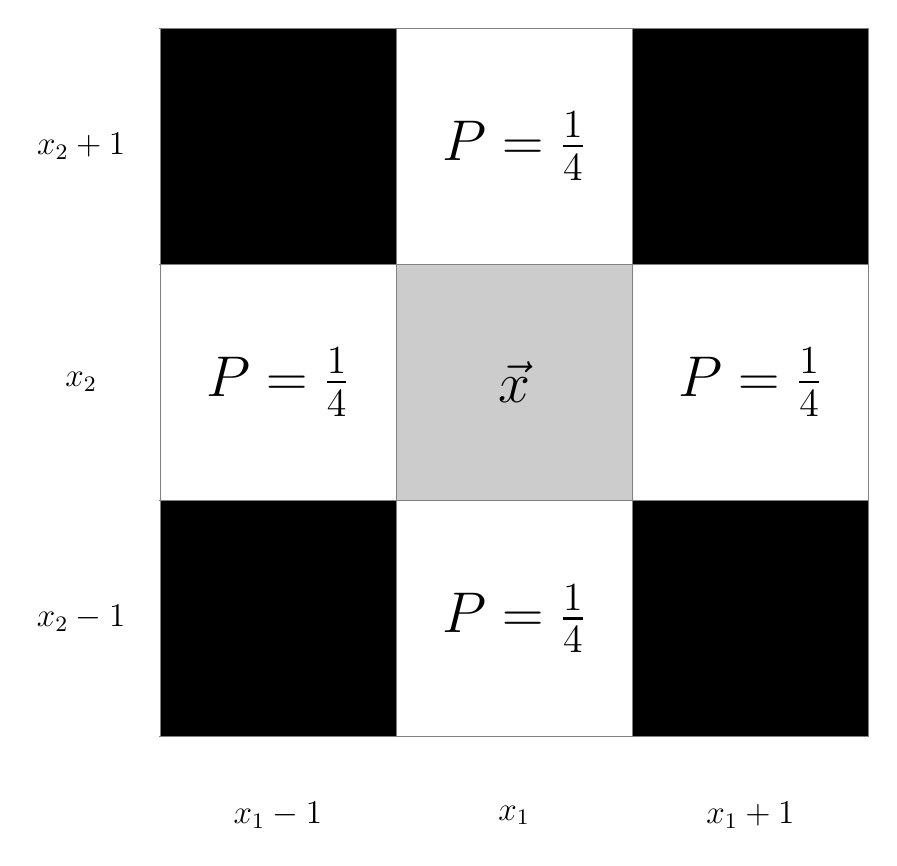
\begin{tikzpicture}

\fill[black] (-3,-3) rectangle (0,0);
\fill[black] (3,3) rectangle (6,6);
\fill[black] (-3,3) rectangle (0,6);
\fill[black] (3,-3) rectangle (6,0);
\fill[gray!40!white] (0,0) rectangle (3,3);

\draw[step=3cm,gray,very thin] (-3.01,-3.01) grid (6,6);

% \node at (1.5,1.5) {\huge$(x_1,x_2)$};
\node at (1.5,1.5) {\huge$\vec{x}$};
\node at (-1.5,1.5) {\huge$P=\frac{1}{4}$};
\node at (1.5,-1.5) {\huge$P=\frac{1}{4}$};
\node at (1.5,4.5) {\huge$P=\frac{1}{4}$};
\node at (4.5,1.5) {\huge$P=\frac{1}{4}$};

\node at (-4,4.5) {\large\bf$x_2+1$};
\node at (-4,1.5) {\large\bf$x_2$};
\node at (-4,-1.5) {\large\bf$x_2-1$};

\node at (-1.5,-4) {\large\bf$x_1-1$};
\node at (1.5,-4) {\large\bf$x_1$};
\node at (4.5,-4) {\large\bf$x_1+1$};

\end{tikzpicture}
\caption{Probability of next step in the 2D random walk}\label{2DrandomWalkProbs.fig}
\end{figure}
    
\paragraph{Model}
Ultimately, our goal is to find a form of Fick's Law using $p(\vec{x},t) = P[\vec{x},t]$, of which the above description is setup for. Note that we can replace $t$ with $t+1$ or any other $t$ without loss of generality due to the memoryless property of 2D random walk.

We begin by describing $P[\vec{x},t+1]$ using our knowledge of the probabilities of where it may be at the prior time step $t$.

\begin{align*}
    P\left[\vec{x}, t+1\right] =&\quad\, \frac{1}{4}P\left[\begin{bmatrix} x_1+1\\x_2 \end{bmatrix}, t\right]\\
    &+\frac{1}{4}P\left[\begin{bmatrix} x_1-1\\x_2 \end{bmatrix}, t\right]\\
    &+\frac{1}{4}P\left[\begin{bmatrix} x_1\\x_2+1 \end{bmatrix}, t\right]\\
    &+\frac{1}{4}P\left[\begin{bmatrix} x_1\\x_2-1 \end{bmatrix}, t\right]
\end{align*}

In order to develop the parallels to Fick's law, we take the Taylor expansions of each of our probabilities with respect to $t$ for $P\left[\vec{x}, t+1\right]$ and with respect to $x$ for each of the probabilities we've used at time $t$.

First, we take the our target probability and find its first order Taylor expansion with respect to time, and using our $p(\vec{x},t)$ as described earlier.
\begin{align*}
    P\left[\vec{x}, t+1\right] &\approx P\left[\vec{x}, t+1\right] + \nabla^T_t\left(P\left[\vec{x}, t+1\right]\right) (t+1-t) \\
    &= p + \frac{\partial p}{\partial t} \\
    &= p
\end{align*}
Note that we exploit the memoryless property of random walk to reduce $\frac{\partial p}{\partial t}$ to 0, as the probability that a particle performing truly random walk is in a certain location in space is not influenced by time.

Next, we take the second order Taylor expansion of our probabilities of movement in the $x_1$ direction, using similar substitutions as before. Here, $\mathcal{H}(f)$ describes the Hessian of the function $f$. 
\begin{align*}
    P\left[\begin{bmatrix} x_1\pm1\\x_2 \end{bmatrix}, t\right] &\approx p + \nabla^T_{\vec{x}}(p) \left(\begin{bmatrix} x_1\pm1\\x_2 \end{bmatrix} - \vec{x}\right) + \left(\begin{bmatrix} x_1\pm1\\x_2 \end{bmatrix} - \vec{x}\right)^T \mathcal{H}(p)  \left(\begin{bmatrix} x_1\pm1\\x_2 \end{bmatrix} - \vec{x}\right) \\
    &= p + \left(\frac{\partial p}{\partial x}\right)^T \begin{bmatrix} \pm1\\0 \end{bmatrix} + \begin{bmatrix} \pm1\\0 \end{bmatrix}^T \begin{bmatrix}
        \frac{\partial^2 p}{\partial x_1^2} & \frac{\partial p}{\partial x_2 x_1} \\
        \frac{\partial p}{\partial x_1 x_2} & \frac{\partial^2 p}{\partial x_2^2}
    \end{bmatrix} \begin{bmatrix} \pm1\\0 \end{bmatrix} \\
    &= p \pm \left(\frac{\partial p}{\partial x}\right)^T \begin{bmatrix} 1\\0 \end{bmatrix} + \frac{\partial^2 p}{\partial x_1^2}
\end{align*}

Similarly, we take the second order Taylor expansion for probabilities in the $x_2$ direction.
\begin{align*}
    P\left[\begin{bmatrix} x_1\\x_2\pm1 \end{bmatrix}, t\right] &\approx 
    p + 
    \nabla^T_{\vec{x}}(p) \left(\begin{bmatrix} x_1\\x_2\pm1 \end{bmatrix} - \vec{x}\right) + \left(\begin{bmatrix} x_1\\x_2\pm1 \end{bmatrix} - \vec{x}\right)^T \mathcal{H}(p)  \left(\begin{bmatrix} x_1\\x_2\pm1 \end{bmatrix} - \vec{x}\right) \\
    &= p \pm \left(\frac{\partial p}{\partial x}\right)^T \begin{bmatrix} 0\\1 \end{bmatrix} + \begin{bmatrix} 0\\1 \end{bmatrix}^T \begin{bmatrix}
        \frac{\partial^2 p}{\partial x_1^2} & \frac{\partial p}{\partial x_2 x_1} \\
        \frac{\partial p}{\partial x_1 x_2} & \frac{\partial^2 p}{\partial x_2^2}
    \end{bmatrix} \begin{bmatrix} 0\\1 \end{bmatrix} \\
    &= p \pm \left(\frac{\partial p}{\partial x}\right)^T \begin{bmatrix} 0\\1 \end{bmatrix} + \frac{\partial^2 p}{\partial x_2^2}
\end{align*}

Now, we combine all of the above into our original expression
\begin{align*}
    p =&\quad\, \frac{1}{4}\left(p + \left(\frac{\partial p}{\partial x}\right)^T \begin{bmatrix} 1\\0 \end{bmatrix} + \frac{\partial^2 p}{\partial x_1^2}\right)\\
    &+\frac{1}{4}\left(p - \left(\frac{\partial p}{\partial x}\right)^T \begin{bmatrix} 1\\0 \end{bmatrix} + \frac{\partial^2 p}{\partial x_1^2}\right)\\
    &+\frac{1}{4}\left(p + \left(\frac{\partial p}{\partial x}\right)^T \begin{bmatrix} 0\\1 \end{bmatrix} + \frac{\partial^2 p}{\partial x_2^2}\right)\\
    &+\frac{1}{4}\left(p - \left(\frac{\partial p}{\partial x}\right)^T \begin{bmatrix} 0\\1 \end{bmatrix} + \frac{\partial^2 p}{\partial x_2^2}\right)
\end{align*}
We note how the first order terms cancel out and proceed to further simplify. Take note of the use of the Laplacian operator $\nabla^2$.
\begin{align*}
    p &= p + \frac{1}{4}\left(\frac{\partial^2 p}{\partial x_1^2}+\frac{\partial^2 p}{\partial x_1^2}+\frac{\partial^2 p}{\partial x_2^2}+\frac{\partial^2 p}{\partial x_2^2}\right) \\
    0 &= \frac{1}{2}\left(\frac{\partial^2 p}{\partial x_1^2}+\frac{\partial^2 p}{\partial x_2^2}\right)\\
    \nabla^2 p &= \frac{\partial^2 p}{\partial x_1^2}+\frac{\partial^2 p}{\partial x_2^2}\\
    \nabla^2 p &= 0
\end{align*}
We note that this final result to be (as expected) the solution to Fick's second law in the special case of the diffusion (or random walk, in our case) being independent of time, also known as Laplace's equation. For a more general result (i.e. not assuming that our particle's position is independent of time), using these same methods we would arrive at the more general statement of Fick's second law
$$\frac{\partial p}{\partial t} = \nabla^2 p$$

To close, while this result was derived for the two-dimensional random walk case, the derivation for n-dimensions should be readily apparent from this case.


\vspace{12pt}


{\it Adapted in part from} \url{http://engineering.dartmouth.edu/~d30345d/courses/engs43/chapter2.pdf}

\subsection{Heavy chain}

\subgroup{4}{Rob Ruigrok}

\paragraph{Description}
This chapter will cover the derivation of the dynamics of a heavy chain with uniform density $\rho$, length $L$ and a point mass on the end with mass $m$. The top of the chain will be suspended on a rolling trolley, where the lateral speed can be controlled. First, we will derive the dynamics, and later go into more detail on the "flatness" of the system and several control inputs.

\paragraph{Model}

An overview of the system is provided in figure \ref{fig:heavychainoverview}. Let $x$ be coordinate along the length of the chain, where the chain is attached to the trolley at $x=L$. The lateral displacement of the chain is denoted by $y(x,t)$. The problem can be made more complex by adding a point mass $m$ to the end of the chain.

\begin{figure}[h]
\label{fig:heavychainoverview}
\centering
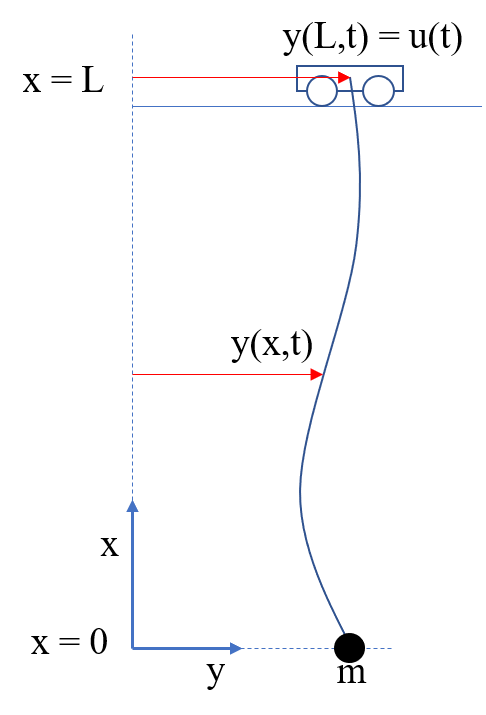
\includegraphics[width = 4cm]{Overview.png}
\end{figure}

The derivation of the dynamics goes largely the same as the derivation of the vibrating spring. Here, however, the tension in the chain will be depending on $x$, and there will now be different boundary conditions linked to the trolley at the top and the attached mass at the bottom. Figure \ref{fig:heavychaindx} illustrates the forces acting on a finite chain element of length $dx$, which is the basis in the derivation of the PDE.\newline

\begin{figure}[h]
\label{fig:heavychaindx}
\centering
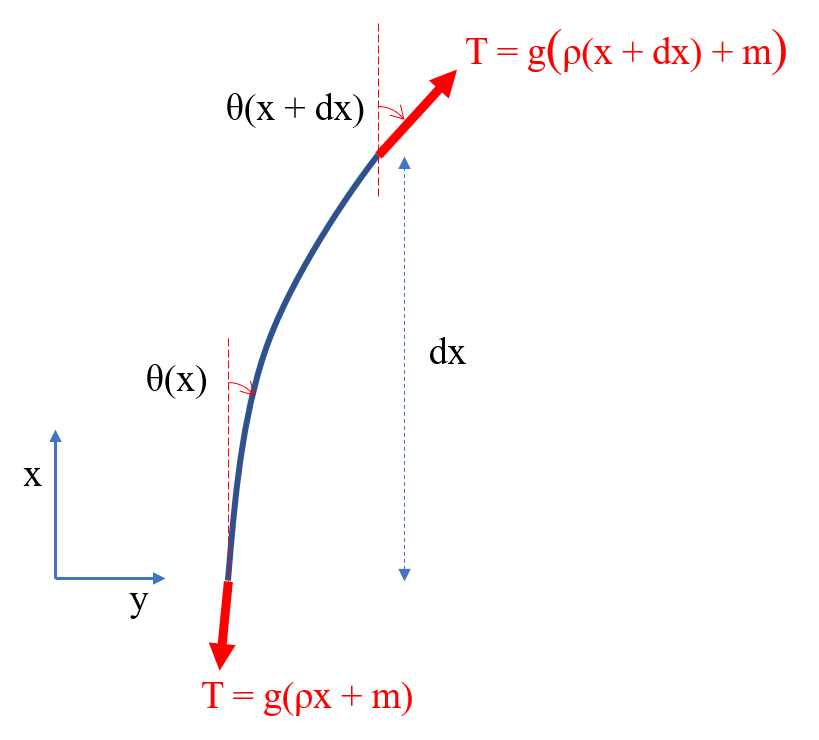
\includegraphics[width = 5cm]{SmallElement.png}
\end{figure}

We start with defining the tension in the chain as a function of $x$:

\begin{equation}
\label{eq:chaintension}
T = (m + x\rho)g
\end{equation}

To analyze the dynamics, we are interested of the lateral component of this tension. When examining an infinitesimal chain element of length $\Delta x$, we are interested in the net lateral force. Instead of defining the force on both sides of element $\Delta x$, we here determining the difference by using a first order Taylor approximation, together with a small angle approximation:

\begin{equation}
\label{eq:chainapprox}
sin(\theta)T \approx tan(\theta)T = \frac{\partial y}{\partial x}T
\end{equation}

\begin{equation}
\label{eq:chainforce}
\Delta F \approx F_x \Delta x = \big[\frac{\partial y}{\partial x}T\big]_x \Delta x
\end{equation}

The lateral motion of an infinitesimal chain element can now be described with Newtons second law of motion, $F = ma$, for which the net force is defined in equation \ref{eq:chainforce}. The mass of the chain element is $\rho \Delta x$, and the acceleration is $\frac{\partial^2 y}{\partial t^2}$

\begin{equation}
\begin{aligned}
    F &= ma \\
    \big[\frac{\partial y}{\partial x}T\big]_x \Delta x &= \rho \Delta x \frac{\partial^2 y}{\partial t^2} \\
    \big[\frac{\partial y}{\partial x} (m + x\rho)g \big]_x &= \rho \frac{\partial^2 y}{\partial t^2}
\end{aligned}
\end{equation}

When there is no mass suspended to end of the chain, the dynamics can be further written out:

\begin{eqnarray}
\label{eq:chainPDE}
    \big[\frac{\partial y}{\partial x} x \rho g \big]_x &=& \rho \frac{\partial^2 y}{\partial t^2} \\
    g \big[\frac{\partial y}{\partial x} x \big]_x &=& \frac{\partial^2 y}{\partial t^2} \\
    g \big[x \frac{\partial^2 y}{\partial x^2} + \frac{\partial y}{\partial x} \big] &=& \frac{\partial^2 y}{\partial t^2}
\end{eqnarray}
with boundary condition: $y(L,t) = u(t) $.


\paragraph{Solving the PDE}
\bigskip
\emph{\textbf{TODO: move part of it to control section
}}\bigskip

It is difficult to directly find a solution for the partial differential equation in equation~5\ref{eq:chainPDE}). For this particular problem, we assume that we know that we can rewrite to a Bessel function. Bessel functions are mainly used to describe wave propagation, and have the following format, where $\alpha$ denotes the order of the Bessel function:

\begin{equation}
\label{eq:Bessels}
x^2\frac{d^2 y}{dx^2} + x\frac{dy}{dx} + (x^2 - \alpha^2)y = 0
\end{equation}

In order to make the formulation in equation \ref{eq:chainPDE} fit this a zero-order Bessel function, we have to do certain changes of variables and convert the problem to the Laplace domain. In the Laplace domain, we can find solutions for our type of Bessel function, after which we need to transform it back to the time domain and reverse the variable changes. \newline

\paragraph{Step 1: substitution}

First step, do a substitution with $p = 2\sqrt{\frac{x}{g}}$. This will change the dependency from y(x,t) to y(p,t). Use the chain rule and find fill out the new values:

\begin{equation}
\label{eq:ChainRule}
\begin{aligned}
\frac{\partial p}{\partial x} &= \frac{1}{g}\bigg(\frac{x}{g}\bigg)^{-\frac{1}{2}} = \frac{1}{g\sqrt{\frac{x}{g}}} = \frac{2}{gp}\\
\frac{\partial y}{\partial x} &=  \frac{\partial y}{\partial p} \frac{\partial p}{\partial x} + \frac{\partial y}{\partial t} \cancelto{0}{\frac{\partial t}{\partial x}} = \frac{\partial y}{\partial p} \frac{2}{gp}
\end{aligned}
\end{equation}

When we fill everything out in the left part of equation \ref{eq:chainPDE}, we get the following expression:

\begin{equation}
\label{eq:chaincombination1}
\begin{aligned}
g \frac{\partial}{\partial x}\big[\frac{\partial y}{\partial x} x \big] &= g \frac{\partial}{\partial x}\big[\frac{\partial y}{\partial p} \frac{2}{gp} \frac{1}{4}gp^2 \big] = g \frac{\partial}{\partial x}\big[\frac{\partial y}{\partial p} \frac{p}{2} \big] \\
&= g \frac{\partial}{\partial p}\big[\frac{\partial y}{\partial p} \frac{p}{2} \big]\frac{\partial p}{\partial x} = g \big[\frac{\partial^2 y}{\partial p^2} \frac{p}{2} + \frac{1}{2} \frac{\partial y}{\partial p}\big] \frac{2}{gp} \\
&= \frac{\partial^2 y}{\partial p^2} + \frac{1}{p} \frac{\partial y}{\partial p}
\end{aligned}
\end{equation}

So the total equation can be written as:
\begin{eqnarray}
\label{eq:chaincombination2}
 g \big[\frac{\partial y}{\partial x} x \big]_x - \frac{\partial^2 y}{\partial t^2} &=& 0 \\
  \frac{\partial^2 y}{\partial p^2} + \frac{1}{p} \frac{\partial y}{\partial p} - \frac{\partial^2 y}{\partial t^2} &=& 0 \\
 p \frac{\partial^2 y}{\partial p^2} +
  \frac{\partial y}{\partial p} - p \frac{\partial^2 y}{\partial t^2} &=& 0
\end{eqnarray}

\paragraph{Step 2: transform to Laplace domain}

When converting the from the time domain, we use the following notation:
\begin{center}
$y(x,t) \xrightarrow{\mathcal{L}} Y(x,s)$
\end{center}
Further, to get the Laplace transform in the desired format, we require that the systems is initially \textit{at rest}, which means that $y(x,0)=0$ and $\dot{y}(x,0)=0$.

\begin{equation}
\label{eq:heavychainlaplace}
\begin{aligned}
 p \frac{\partial^2 y(x,t)}{\partial p^2} +
  \frac{\partial (x,t)}{\partial p} - p \frac{\partial^2 y(x,t)}{\partial t^2} = 0 \\
  \xrightarrow{\mathcal{L}}
 p \frac{\partial^2 Y(x,s)}{\partial p^2} +
  \frac{\partial Y(x,s)}{\partial p} - p s^2 Y(x,s) = 0
\end{aligned}
\end{equation}

NEW CHANGE OF VARIABLES (did it myself on paper, still need to isert)\newline
Bessel function!




\section{Manipulation of partial differential equations}
%----------------------------------------------------------------------

\subsection{Weak formulation}
% ***********************************************************************************
% Pure LaTeX part to be inserted in a document (be careful of depencies of packages & commands
% Prepared by Xin Peng and Hongbei Chen under the supervision of Arnaud de La Fortelle
% Fall 2017
% weak formulation Dirichlet of the modeling part
% ***********************************************************************************
\subgroup{3} {Xin Peng and Hongbei Chen}


\paragraph{Objective}

Weak formulations are important tools for the analysis of mathematical equations that permit the transfer of concepts of linear algebra to solve problems in other fields such as partial differential equations. In a weak formulation, an equation is no longer required to hold absolutely and has instead weak solutions only with respect to certain "test vectors" or "test functions". This is equivalent to formulating the problem to require a solution in the sense of a distribution.

Take Poisson's equation as a example. Our aim is to solve this Poisson's equation
$$-\Delta u= f\eqno(1.1)$$
on a domain $\Omega \subset R^d$,$u=0$ on its boundary.\\
Suppose $u$ is continuously differentiable in continental space $R^{2}$, test it with differentiable functions $v$ and integral, we get

$$\int_\Omega \left ( \nabla^2u \right )v\ud x=\int_\Omega fv\ud x\eqno(1.2)$$
We can make the left side of this equation more symmetric by integration by parts using Green's identity and assuming that $v=0$ on $\partial \Omega $
$$-\int _\Omega \left ( \nabla^2u \right )v\ud x= -\int _{\partial\Omega }\left ( \nabla u \right )v\ud s+\int _\Omega \nabla u \nabla v\ud x\eqno(1.3)$$

$$-\int _\Omega \left ( \nabla^2u \right )v\ud x=\int _\Omega \nabla u \nabla v\ud x\eqno(1.4)$$
The equation 1.4 is what is usually called the weak formulation of Poisson's equation. As we can see, weak formulations are partial differential equations testing with "test vectors" or "test functions" and then integral both side of equations. This transformation sacrifices the smoothness of solution. Since a large number of differential equations used to describe the phenomena in the real world do not have enough smooth solutions to solve such equations can only use weak formulation.\\

\paragraph{Demonstration}

A Dirichlet problem is the problem of finding a function which solves a specified partial differential equation in the interior of a given region that takes prescribed values on the boundary of the region. We take a PDE for example.\\


We consider $f$ a continuous function on $\Omega$ of sumtable square and $u$ the solution of the following partial derivative equation on $\Omega$
$$-\Delta u+k^{2} u=f\eqno(2.1)$$
With the condition at the edge $u=0$ on $\partial\Omega$. This can also be rewritten $u\subset V _{0}$. This condition at the edge is called the Dirichlet condition. We prove that there exists a unique solution to this PDE problem using the Lax-Milgram theorem.\\

Let $u\subset V _{0}$ be arbitrary. Multiply the two parts of the previous equation by $v$ then sum to the domain $\Omega$, since $v$ and $f$ are both summable square on this domain. Equation:
$$-\int _\Omega \Delta uv\ud w + k^2\int _\Omega uv\ud w = \int _\Omega vf\ud w\eqno(2.2)$$
We can make the left side of this equation more symmetric by integration by parts using Green's identity:
$$-\int _\Omega v\Delta u\ud w=-\int _{\partial \Omega }v\nabla u\ud s+\int _\Omega \left ( \nabla u \nabla v \right )\ud w\eqno(2.3)$$
In this formulation, $v=0$ on $\partial \Omega $ $(v\subset V _{0})$.Thus $\int _{\partial \Omega }v\nabla u\ud s=0$.
$$\int _\Omega \left ( \nabla u \nabla v \right )\ud w+ k^2\int _\Omega uv\ud w = \int _\Omega vf\ud w\eqno(2.4)$$
If u is twice differentiable, there is equivalence between this formulation and that of the initial problem given in the hypothesis section(Because we used to integral both side of equation). Then the solution of the weak formulation is the same as the initial solution. We can therefore solve the weak formulation instead of solving the initial problem.





\subsection{}
%section 2.3.2

\subsection{}
%section 2.3.3

\subsection{Example of solving the 2D heat diffusion}
% ***********************************************************************************
% Pure LaTeX part to be inserted in a document (be careful of depencies of packages & commands
% Prepared by Qingan Zhao under the supervision of Arnaud de La Fortelle
% Fall 2017
% Example of solving the 2D heat diffusion subsection of the modeling part part
% ***********************************************************************************

\subgroup{2}{Qingan Zhao}

\paragraph{Description}
Now consider a retangular plane (length: a; width: b) with 2 boundaries that have no heat transfer (i.e., $T(x, 0)=f(x);\ T(x, b)=g(x)$). The other two boundaries have fixed temperature ($T(0, y)=T(a, y)=0$). We would like to solve the PDE under the stationary state (i.e., $\ud T/\ud t=0$). The diagram of the system is shown in Figure~\ref{heatSolSystem.fig}.
\begin{figure}[htb]
	\centering
	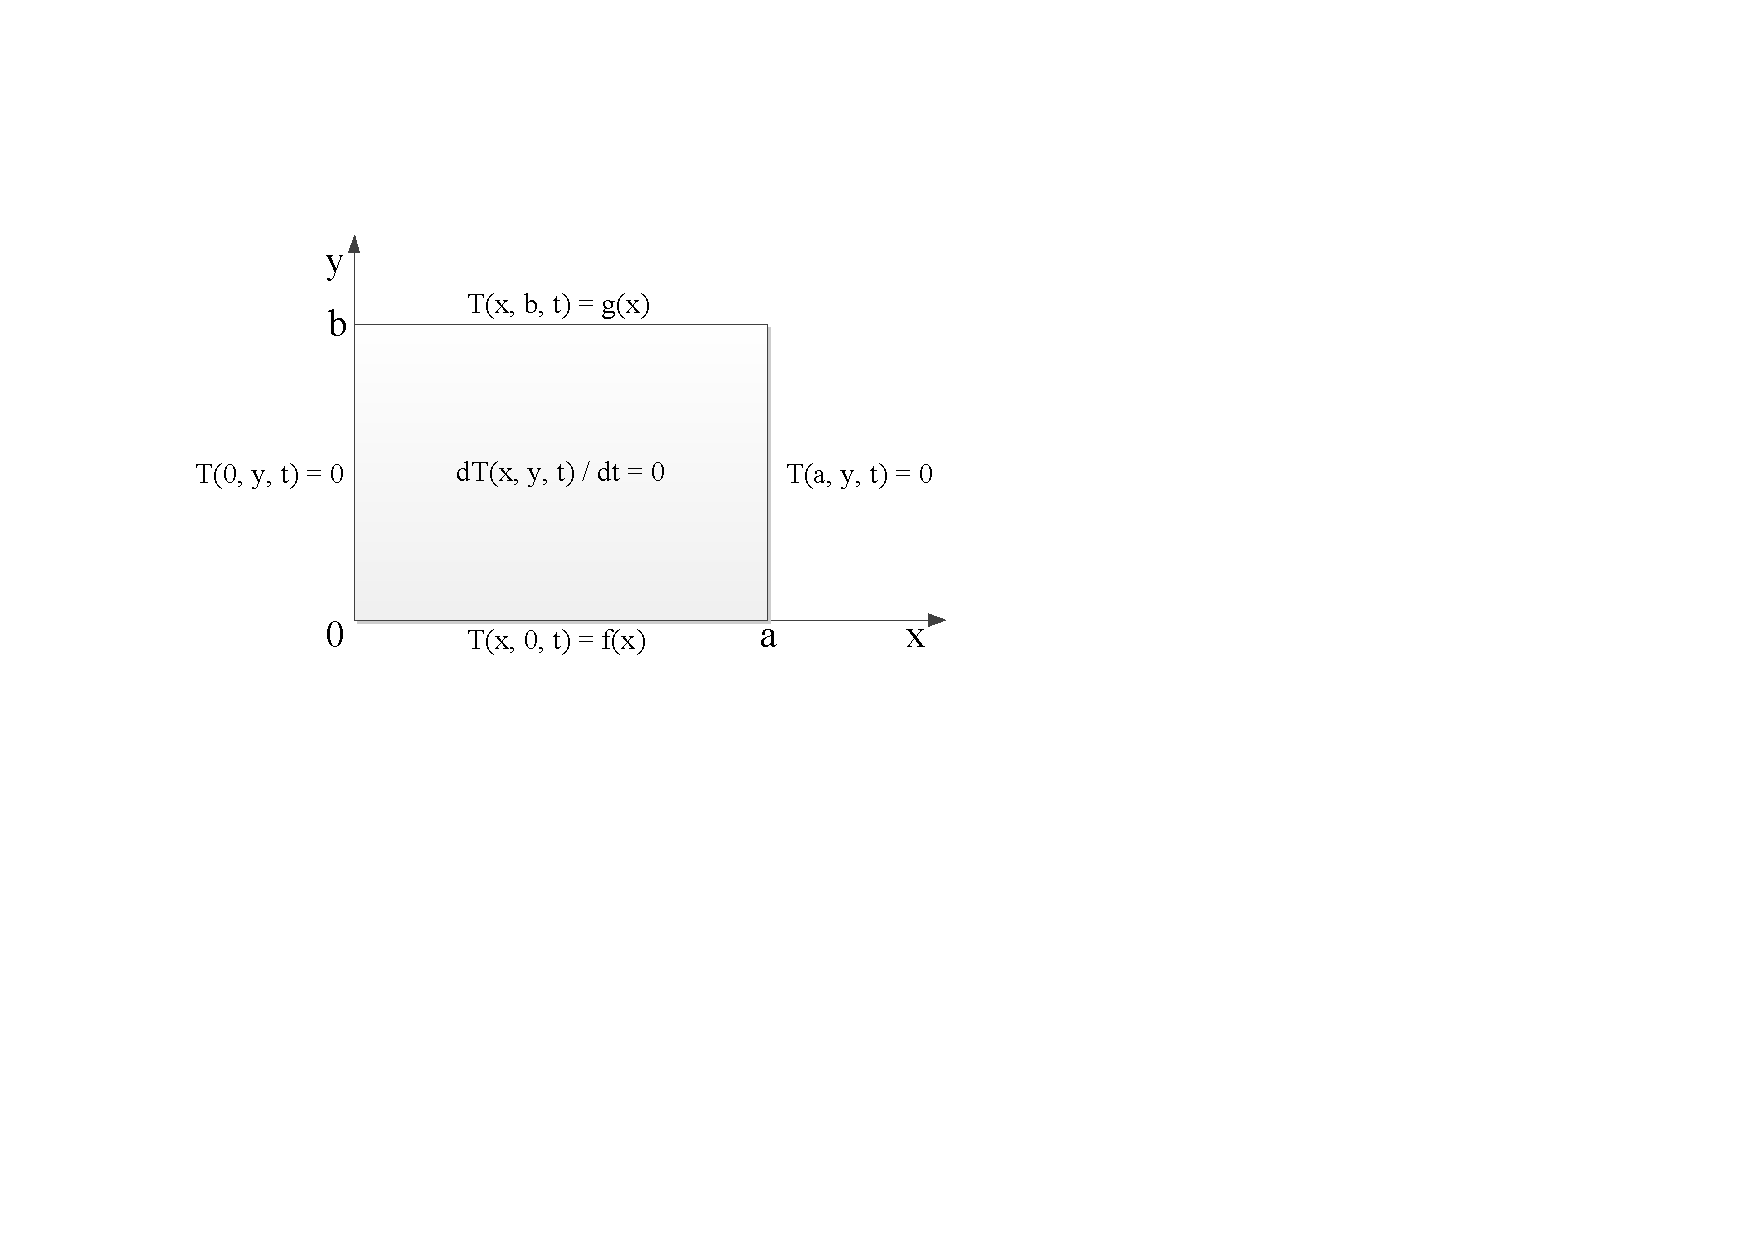
\includegraphics[width=10cm]{2dHeatSolDescription.pdf}       
	\caption{System description of the example}\label{heatSolSystem.fig}
\end{figure}

\paragraph{PDE and boundary conditions}
From Section 2.2.2 we have already known that the 2D heat equation is:
\begin{equation}
\frac{\partial T}{\partial t}=a^2\left(\frac{\partial ^2 T}{\partial x^2}+\frac{\partial ^2 T}{\partial y^2}\right)\ \ \ \ where\ a=\sqrt{\frac{k}{c\rho}}
\end{equation}


The boundary conditions of this problem are as follows:

\begin{equation}\label{2DHeatBound1.eq}
T(x,0,t)=f(x)
\end{equation}
\begin{equation}\label{2DHeatBound2.eq}
T(x,b,t)=g(x)
\end{equation}
\begin{equation}\label{2DHeatBound3.eq}
T(0, y, t)=0
\end{equation}
\begin{equation}\label{2DHeatBound4.eq}
T(a, y, t)=0
\end{equation}
\begin{equation}
\frac{\ud T}{\ud t}=0
\end{equation}

\paragraph{Solution}
Since the system is under the stationary state ($\ud T/\ud t=0$), $T(x,y,t)$ can be expressed as $T(x,y)$, and the PDE can be written as:
\begin{equation}
\frac{\partial^2T}{\partial x^2}+\frac{\partial^2T}{\partial y^2}=0
\end{equation}

We could sperate the variables by express $T(x,y)$ as $X(x)Y(y)$. Then the PDE can be written as:
\begin{equation}
X''(x)Y(y)+X(x)Y''(y)=0
\end{equation}

Since $X(x)Y(y)$ is not identically zero, divide both sides by $X(x)Y(y)$ gives:
\begin{equation}
\frac{X"(x)}{X(x)}+\frac{Y"(y)}{Y(y)}=0
\end{equation}

Since the two parts of the left side are independent, the following equations can be drawn ($\lambda$ is a constant):
\begin{align}
X"(x)+\lambda X(x)=0\\
Y"(y)-\lambda Y(y)=0
\end{align}

Moreover, the boundary conditions Equations~(\ref{2DHeatBound3.eq})-(\ref{2DHeatBound4.eq}) give:
\begin{align}
X(0)Y(y)=0\\
X(a)Y(y)=0
\end{align}

Since $Y(y)$ is not identically zero, we can obtain the following:
\begin{align}
X(0)=0\\
X(a)=0
\end{align}

Hence, the problem becomes solving two indenpendent ordinary differential equations. We know that only when $\lambda=\frac{n^2\pi^2}{a^2}\ (n=1,2,3,...)$, the problem has the following solution:
\begin{equation}
X_n(x)=sin\frac{n\pi x}{a}
\end{equation}
\begin{equation}
Y_n(y)=a_ne^{\frac{n\pi}{a}y}+b_ne^{-\frac{n\pi}{a}y}
\end{equation}

Hence, the solution can be expressed as:
\begin{equation}
T(x,y)=\sum_{n=1}^{\infty}(a_ne^{\frac{n\pi}{a}y}+b_ne^{-\frac{n\pi}{a}y})sin\frac{n\pi x}{a}
\end{equation}

Given the other two boundary conditions Equations~(\ref{2DHeatBound1.eq})-(\ref{2DHeatBound2.eq}), $a_n$ and $b_n$ can be solved using the following 2 equations:
\begin{equation}
a_n+b_n=\int_{0}^{a}f(x)sin\frac{n\pi}{a}xdx
\end{equation}
\begin{equation}
a_ne^{\frac{n\pi}{a}b}+b_ne^{-\frac{n\pi}{a}b}=\int_{0}^{a}g(x)sin\frac{n\pi}{a}xdx
\end{equation}

Thus, the analytical solution of this problem is solved.
















\thispagestyle{empty}
%----------------------------------------------------------------------
\chapter{Simulation}
\label{simulation.chap}
%----------------------------------------------------------------------

\section{Objectives}
%----------------------------------------------------------------------
The objective is to obtain numerical data (often the successive states of the system), to visualize these data, to build meaningful statistics and finally to link the results with theoretical considerations. Best would be to compare simulations with analytical results, but this may prove infeasible and then more analysis is required to compare theory and simulations.

\section{Simulation examples}
%----------------------------------------------------------------------
\subsection{Forward Euler simulation of the 1D heat equation}
% ***********************************************************************************
% Pure LaTeX part to be inserted in a document (be careful of depencies of packages & commands)
% Prepared by XXX and YYY under the supervision of Arnaud de La Fortelle
% Fall 2017
% 1D heat diffusion subsection of the simulation part
% ***********************************************************************************

\subgroup{1}{Lin Yang and Bradley Cage}

\paragraph{Model presentation}

\begin{figure}[htb]
	\centering
	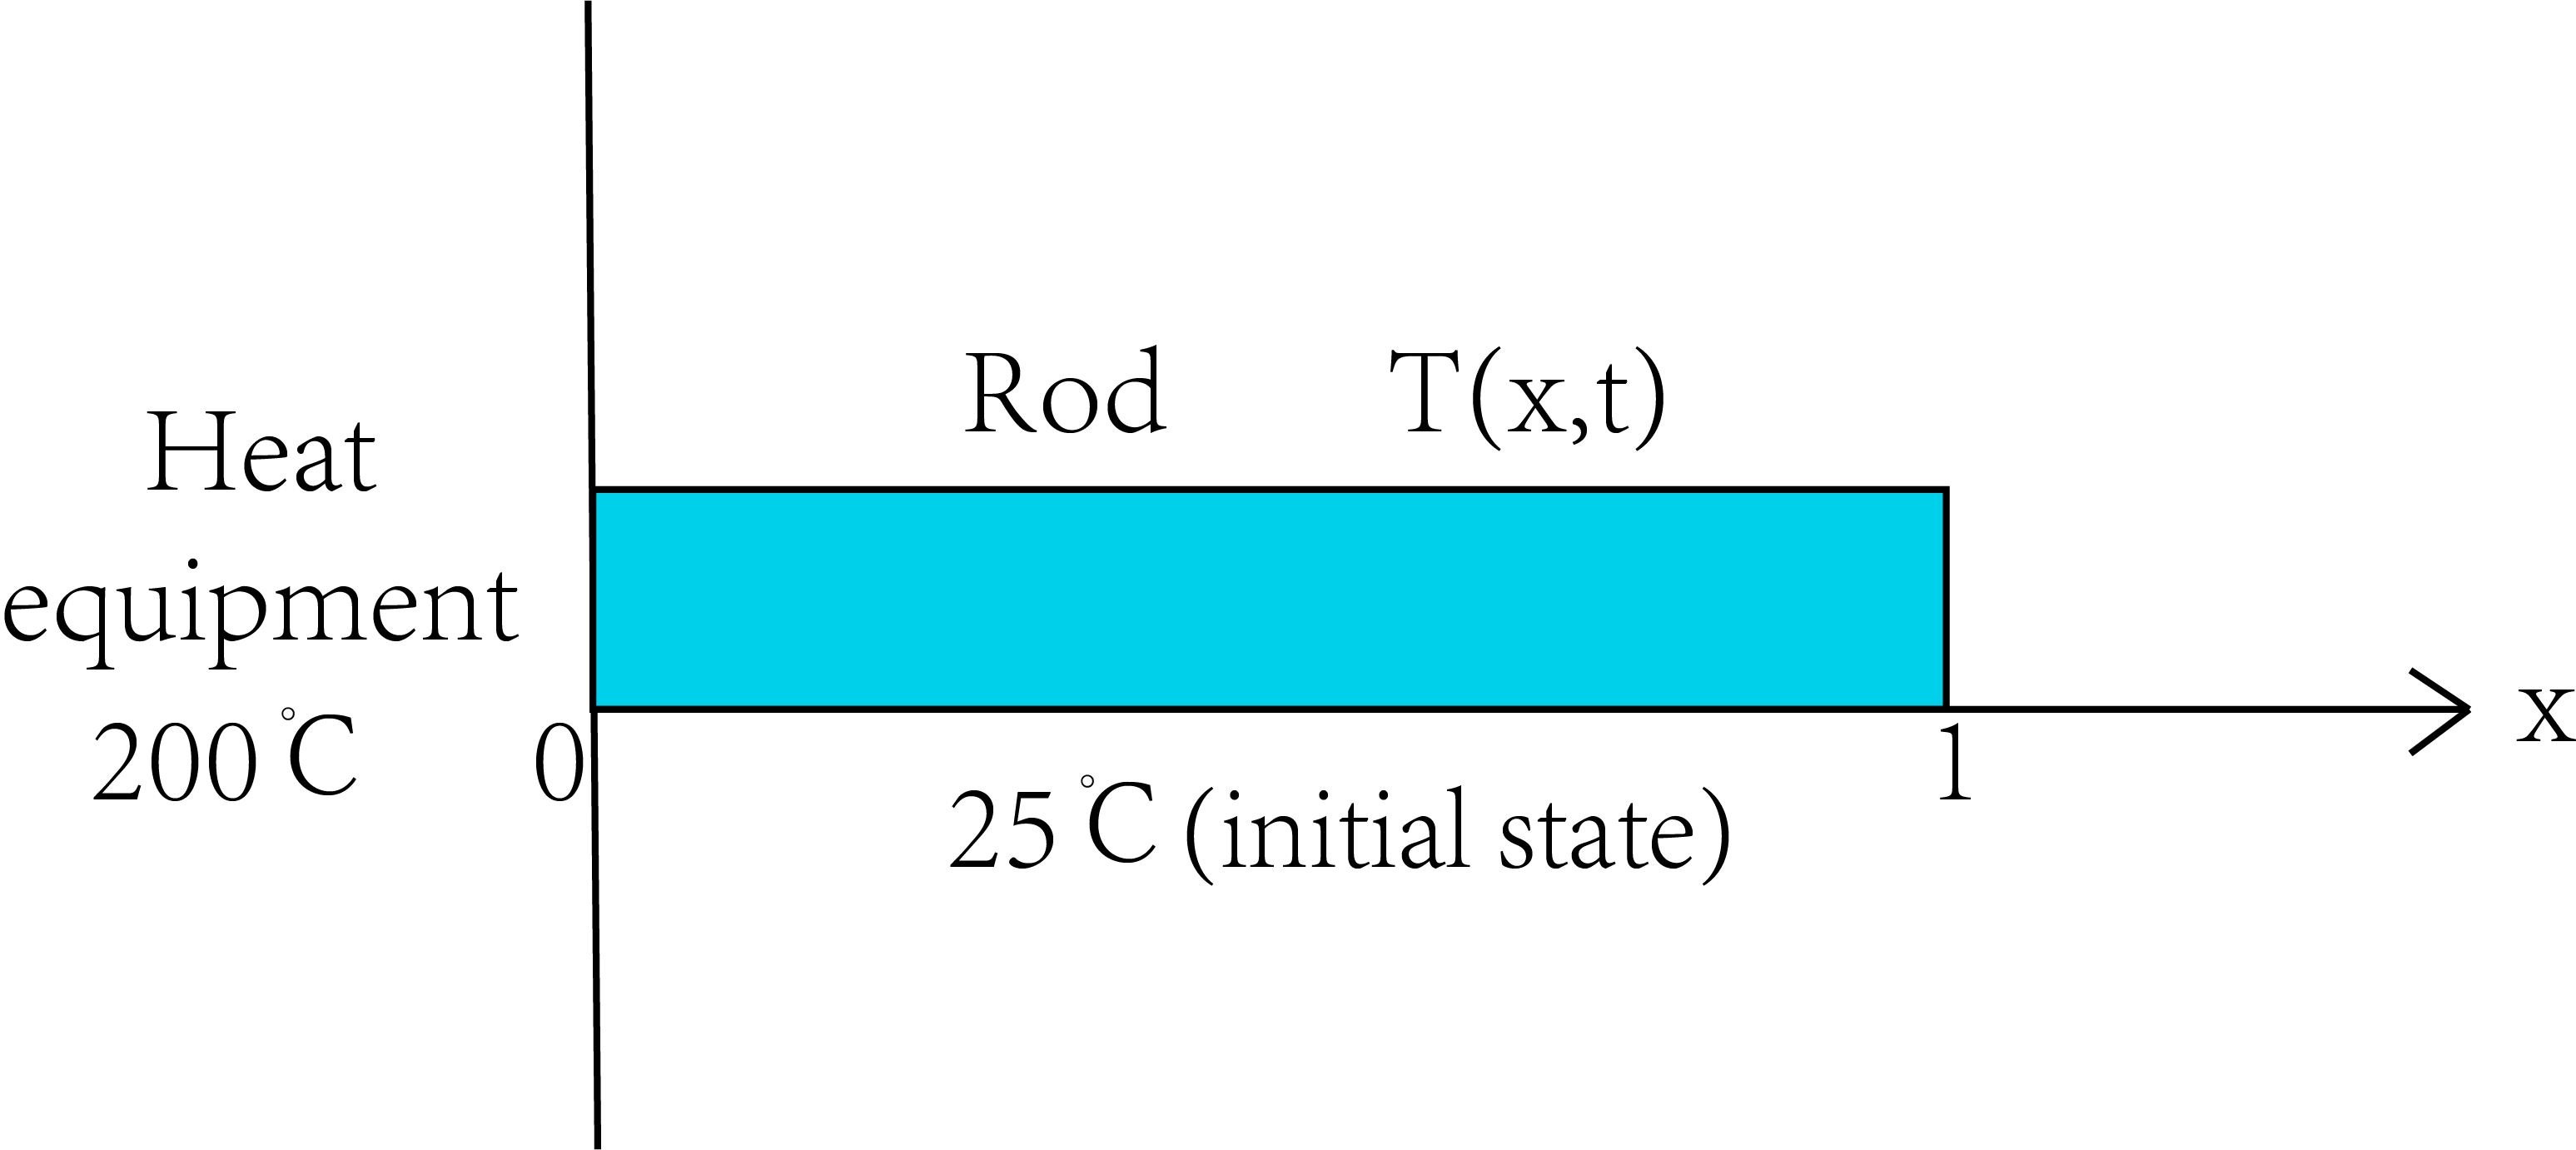
\includegraphics[width=8cm]{Figures/Heat1D_model.png}       
	\caption{The heated rod system, with the temperature at any point given by $T(x,t)$ }
	\label{Heat1D_model.fig}
\end{figure}

Our system is comprised of a rod fixed to a heated wall kept at constant temperature. The length of the rod is arbitrarily taken as 1m. The initial temperature of the rod is in equilibrium with the ambient temperature at 25$^{\circ} $C and the temperature of the wall is 200$^{\circ} $C.  We represent temperature at a point on the rod at some time with the function $T(x,t)$. Note that the rod is thin with respect to its length, thus is modeled as a 1D system, that is, temperature is solely a function of rod position and time. The goal of this simulation is to show the variations in temperature of various points on the rod over time. 

We take our initial state as:
\begin{itemize}
	\item $T(0,t)=200 ^{\circ}$C
    \item $T(x,t)=25 ^{\circ}$C, $x\ne 0$
\end{itemize}

\noindent The partial differential equation of the 1D heat propagation:
\begin{equation}
 \frac{\partial T}{\partial t} = \alpha \frac{\partial^2 T}{\partial x^2}
\end{equation}
\noindent We explicitly state that $u(\cdot)$ is a function of $x$ and $t$
\begin{equation}
 \frac{\partial} {\partial t}T(x,t) = \alpha \frac{\partial^2}{\partial x^2}T(x,t)
\end{equation}
\noindent We use a finite difference approximation to get compute the derivatives in space and time
\begin{equation}
\frac{T_{i}^{N+1}-T_{i}^{N}}{\Delta t} =\alpha\frac{T_{i+1}^{N}-2T_{i}^{N}+T_{i-1}^{N}}{\Delta x^2}
\end{equation}

\noindent Rearranging we reach the final form we need for our Forward Euler approximation. Note that the quantity $\alpha\frac{\Delta t}{\Delta x^2}$ is Fourier's number, with $\alpha$ being the thermal diffusivity of a material. In the following simulations, we arbitrarily choose Aluminium with $\alpha = 9.7e-5$.

\begin{equation}
T_{i}^{N+1}=T_{i}^{N}+\alpha\frac{\Delta t}{\Delta x^2}\big[ {T_{i+1}^{N}-2T_{i}^{N}+T_{i-1}^{N}}\big]
\end{equation}

\paragraph{Implementation}
We provide an implementation in Matlab. 

\begin{lstlisting}[language=Matlab, caption=Forward Euler and Plotting in MATLAB]

  % Values arbitrarily chosen. It's a useful exercise to vary these and look at the results
  T_final = 300;
  N_t = 2000;
  X_final = 1;
  N_x = 100;
  
  % Calculate time and x steps based on sampling size and # of samples
  T = linspace(0, T_final, N_t+1);
  X = linspace(0, X_final, N_x+1);
  dt = T(2) - T(1);  % Calculate delta t
  dx = X(2) - X(1);  % Calculate delta x

  alpha = 9.7e-5; % Thermal diffusivity of Aluminium in m^2/s
  Fo = (alpha*dt)/(dx^2); % Fouriers number = diffusive transport rate/storage rate
 
  % Define your initial condition here. This could be some function IC(x),
  %  however for simplicity's sake we take a rod with a uniform temperature
  %  and in contact with a hot plate at one end
  wall_temp = 200;
  init_temp = 25;
  
  % Initialize the N state and the N-1 state
  u_old = zeros(1, N_x+1); 
  u_old(:) = init_temp;
  u_old(1) = wall_temp;
  u_cur = u_old;
  u_plot = u_old;

  for t = 1:N_t
     for i = 2:N_x
     	 % Forward Euler solution to heat equation
         u_cur(i) = Fo*(u_old(i+1) - 2*u_old(i) + u_old(i-1)) + u_old(i);
     end
     u_cur(1) = wall_temp; % Set the left boundary to be our high of 200 
     u_old(:) = u_cur; % We move to the next time step, reset N-1 state
     u_plot = [u_plot; u_cur];
  end

  [X_plot,T_plot] = meshgrid(X,T); % Create 2D meshgrid to create surface plot

  surf(X_plot,T_plot,u_plot,'EdgeColor','none') % Create surface plot
  c = colorbar; % Attach colour bar and create scale
  c.Label.String = 'Temperature [C]';

  xlim([0 1]) % Add axis limits
  xlabel('Distance along rod [m]'); % Add descriptive axis labels
  ylabel('Time [s]');
  zlabel('Temperature [C]')

\end{lstlisting}


 \paragraph{Results}
\noindent We can create plots of the rods temperature as a function of time and position. This gives us insight into how the system evolves as we maintain our constant temperature. 
\begin{figure}[htb]
	\centering
	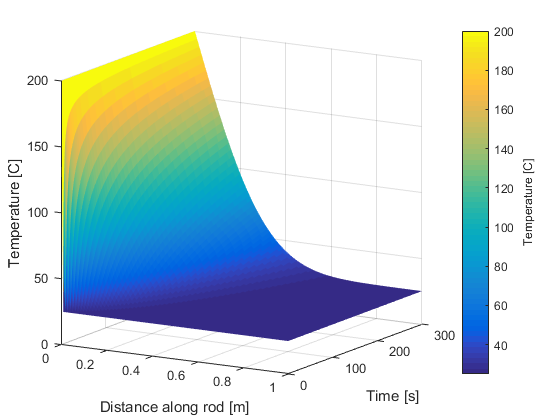
\includegraphics[width=10cm]{Figures/Heat1D_1m.png}       
	\caption{Temperature variation for the whole rod over 300 seconds}
	\label{Heat1D_1m.fig}
\end{figure}

\begin{figure}[htb]

	\centering
	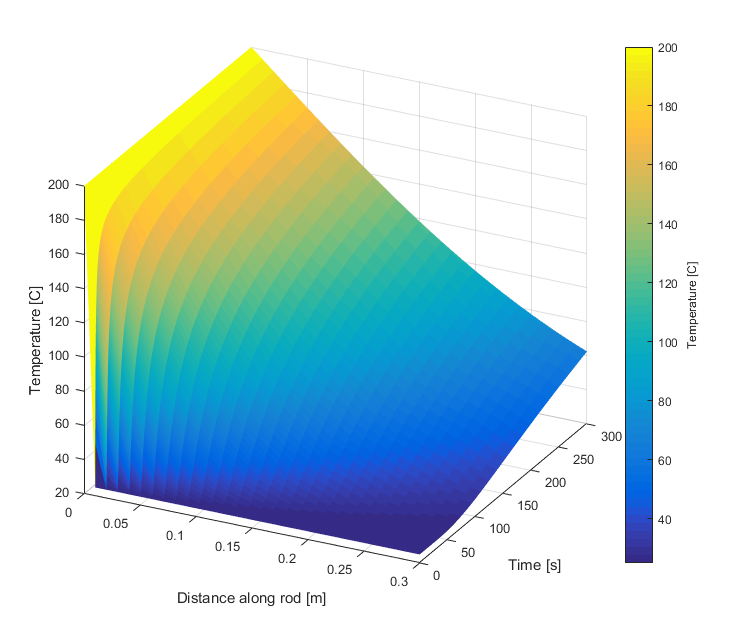
\includegraphics[width=9cm]{Figures/Heat1D_0_3m.png}       
	\caption{Temperature variation for the rod segment with x varies from 0 to 0.3m over 300 seconds}
	\label{Heat1D_0_3m.fig}
\end{figure}
\clearpage
\begin{figure}[!htb]
	\centering
	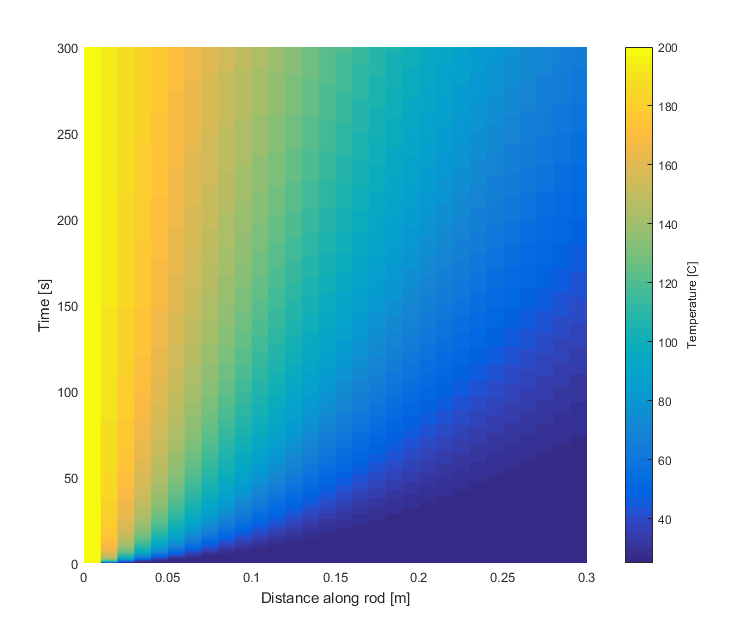
\includegraphics[width=9cm]{Figures/Heat1DTop.png}       
	\caption{Top view of the temperature variation for the whole rod over 300 seconds}
	\label{fig:Heat1D_top}
\end{figure}
 
\paragraph{Interpretation}
The results we obtain are consistent with our model and the physical characteristics. We can see that from the visualization the temperature varies in a logarithmic manner, which is 
consitent with the fact that the Forward Euler scheme approximates the exact mathematical solution to the 2nd order PDE, which takes the form of an exponential. The exact rate at which heat moves through the rod is 
dependent on the thermal conductivity of the material, which makes up part of the exponent (i.e. $e^{-m}$), thus governing the rate. 
We can see pathlines of the heat front evolve over time, especially when looking 
at the system from above. Given enough time, the rod will reach a steady state, which in this example would have the rod rest at a completely uniform temperature, since we have not incorporated any form of heat losses or sinks in the system.

 \paragraph{Conclusion}
Here we have learned that in examining systems such as the heated rod, we can safely analyze it as a 1D system. We were able to discretize the partial differential equations and 
apply a forward Euler simluation to yield phyiscally relevant and meaningful simulations. Through the Matlab visualization, we gain a better understanding of how heat is moving 
through the rod and the system. From the resources and analysis provided, it is trivial to create other initial/boundary conditions and repeat the simulations to garner a deeper
insight into the heat behaviour. This is left as an exercise to the reader. 
 


\subsection{1D vibrating string simulation}
% ***********************************************************************************
% Pure LaTeX part to be inserted in a document (be careful of depencies of packages & commands
% Prepared by XXX and YYY under the supervision of Arnaud de La Fortelle
% Fall 2017
% 2D wave propagation subsection of the modeling part
% ***********************************************************************************

\subgroup{2}{Ruitong Zhu and Qingan Zhao}

\paragraph{Model presentation}
This part is to simulate the vibrating string (i.e., 1D wave equation) and present its displacement with a time-varying image. The string held stationary at both ends and free to vibrate transversely subject only to the restoring forces due to tension in the string. $Figure 1$ shows coordinates and definies symbols for the transverse vibrating string. 

\begin{figure}[htb]
	\centering
	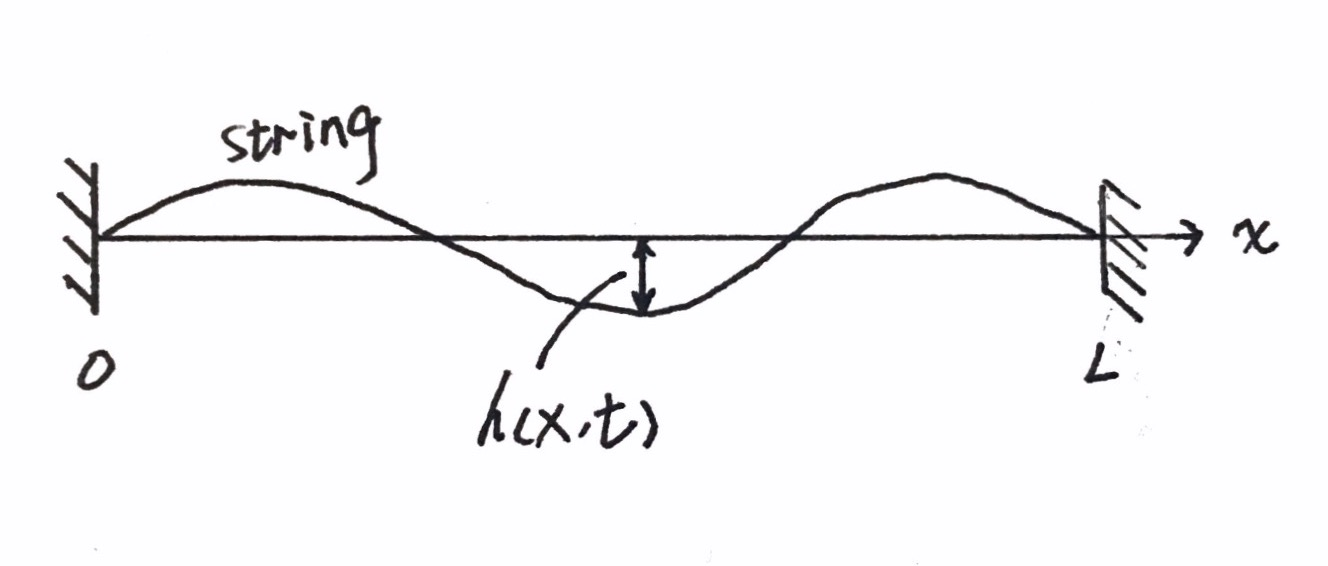
\includegraphics[width=10cm]{string.jpg}       
	\caption{Vibrating String}
\end{figure}

The partial differential equation (PDE) of this problem is given as follow:

\begin{equation}
	\frac{\partial^2 h}{\partial t^2}=a^2\left(\frac{\partial^2 h}{\partial x^2}\right)
\end{equation}

where $h$ is the wave function $h(x,t)$, representing the displacement of the string at position $x$ and time $t$; $a$ is the wave speed which equals to $\sqrt{E/\rho}$.

\paragraph{Implementation}

The simluation is based on Finite Difference Method (FDM). Using second-order central difference at time $t_n$ and position $x_i$, we can get the recurrence equation as follow:

\begin{equation}
\frac{u_{i}^{N+1}-2u_{i}^{N}+u_{i}^{N-1}}{\Delta t^2} = a^2\frac{u_{i+1}^{N}-2u_{i}^{N}+u_{i-1}^{N}}{\Delta x^2}
\end{equation}

Assume the wave speed $a = 1$; the length of the string $L$ is $2$; the maxium time for this simulation is $4$; stepsize $\Delta x$ and $\Delta t$ are both equal to $0.01$. The initial condition and the boundary condition are described as follows:
\begin{eqnarray}
h(x,0)&=&sin(\pi x)\\
\frac{\partial h}{\partial t}\bigg |_{(x,0)}&=&0\\
h(0,t)&=&h(2,t)=0
\end{eqnarray}

Here we offer the implementation in Python:

\begin{python}
	## parameter
	a = 1  ## a coefficient of stiffness
	L = 2  ## The string is constrained at x=0 and x=L.
	T = 4  ## maxium time for this simulation.
	dx = 0.01  ## time step
	dt = 0.01  ## distance step
	N = int(L/dx);
	M = int(T/dt);
	r = (a*dt/dx)**2  ## a parameter

	## initial shape of the string
	def initial(x):
	tmp = math.sin(math.pi*x)
	return tmp
	
	## initial speed of the string
	def speed(x):
	tmp = 0
	return tmp
	
	## Define an array and a blank matrix for later use.
	x = [0]
	h = np.zeros((M+1, N+1))
	
	## t=0, initial condition
	for i in range(N):
	x.append(x[i] + dx)  ## x axis
	h[0,i+1] = initial(x[i+1])  ## displacement of the string
	
	## t=dt, the first itertaion
	for i in range(N-1):
	h[1,i+1] = h[0,i+1] + r* (h[0,i] + h[0,i+2] - 2*h[0,i+1])/2 + dx*speed(x[i+1])
	## displacement of the string
	
	## t=n*dt where n>1
	for j in range(1, M):
	for i in range(N-1):
	h[j+1,i+1] = (h[j,i+2]+h[j,i]-2*h[j,i+1])*r-h[j-1,i+1]+2*h[j,i+1]
	## displacement of the string
	
	t = [0]
	for j in range(M):
	t.append(t[j] + dt)  ## t axis
	
	## Plot the 3D figure.
	fig = plt.figure()
	ax = Axes3D(fig)
	X, T= np.meshgrid(x,t)
	ax.plot_surface(X, T, h, cmap='rainbow')
	ax.set_xlabel('X')
	ax.set_ylabel('T')
	ax.set_zlabel('h')
	plt.show()
	
	## Plot the shape of string at different time
	for i in range(4):
	plt.xlabel(u'x',fontsize=14)
	plt.ylabel(u'h',fontsize=14)
	plt.show()
\end{python}

\paragraph{Results}

The dynamic change of the string is shown in $Figure 2$, ranging from $0\sim 4$.

\begin{figure}[htb]
	\centering
	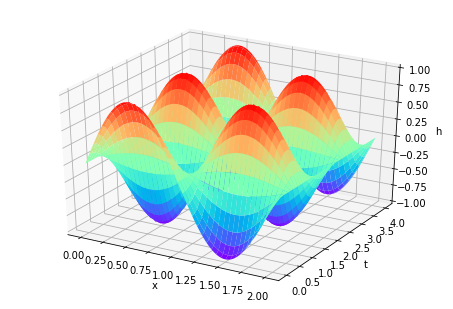
\includegraphics[width=10cm]{string3d.png}       
	\caption{Time-varying Image of the string}
\end{figure}

More specifically, the shapes of the string at different times are shown below:

\begin{figure}[ht]
	\centering
	\begin{minipage}{8cm}
		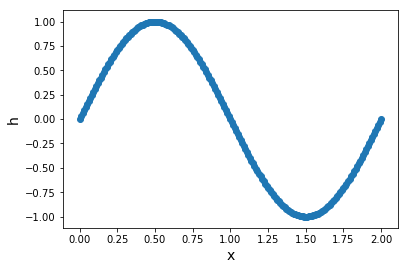
\includegraphics[width=7cm]{string0.png}   
		\caption*{t=0}
		\end{minipage}    
	\begin{minipage}{8cm}
		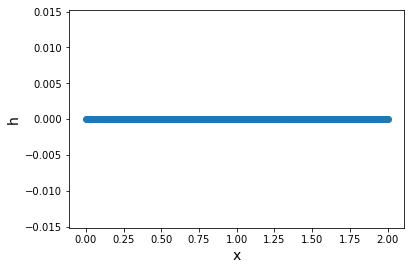
\includegraphics[width=7cm]{string0_5.png}   
		\caption*{t=0.5}
	\end{minipage}  

    \begin{minipage}{8cm}
    	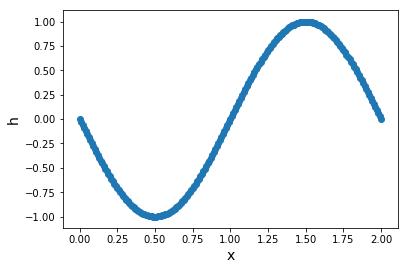
\includegraphics[width=7cm]{string1.png}   
    	\caption*{t=1}
        \end{minipage}  
    \begin{minipage}{8cm}
    	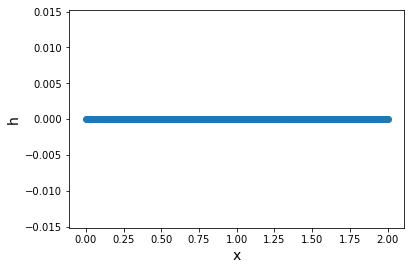
\includegraphics[width=7cm]{string1_5.png}  
    	\caption*{t=1.5} 
    \end{minipage}  
	\caption{Shape of the string at time t}
\end{figure}



\paragraph{Interpretation}

The results are consistent with our expectation. The shape of the string depends on the initial and boundary conditions. In this case, the string is in the shape of a sine wave that changes periodically. 

The initial and boundary conditions can be changed easily at the code by modifying the function $initial()$ and $speed()$. Readers can plot more complicated image with different initial displacement and speed function.

\paragraph{Conclusion}
Finite Difference Method is a practical method to obtain the numerical solution of a Partial Differential Equation. We can learn that it is applicable for one dimentional problems like 1D wave equation and 1D heat equation. It's not difficult to understand but there are some places worth special attention while writing the code. For example, the first iteration needs to be distinguished from other iterations since $t_{N-1}$ is not defined. 



\subsection{1D traffic simulation}
% ***********************************************************************************
% Pure LaTeX part to be inserted in a document (be careful of depencies of packages & commands)
% Prepared by XXX and YYY under the supervision of Arnaud de La Fortelle
% Fall 2017
% 1D LWR traffic model of the simulation part
% ***********************************************************************************

\subgroup{3}{Yue Hu and Carlin Yao}

\paragraph{Model presentation}
What is the model we want to simulate? What do we want to observe? Which is the state space and the dynamics?

\paragraph{Implementation}
Explain the structure of the code. Do not put necessarily all the code (not more than 100 lines) since some routines (functions) can hide efficiently some unnecessary complexity. Provide a code that run (and explicit librairies and dependencies). Ensure your file name is aligned with this part.

 \paragraph{Results}
 Explain the quantities you are studying (i.e. metrics and statistics). Provide good visualization.
 
\paragraph{Interpretation}
Relate these quantities to the model and to theoretical knowledge of the course.

 \paragraph{Conclusion}
 What have we learned? Is everything aligned (theory and practice)? What was difficult? Provide perspectives.
 


\subsection{Random walk in 2D simulation}
% ***********************************************************************************
% Pure LaTeX part to be inserted in a document (be careful of depencies of packages & commands)
% Prepared by XXX and YYY under the supervision of Arnaud de La Fortelle
% Fall 2017
% 12 random walk subsection of the simulation part
% ***********************************************************************************

\subgroup{4}{Yue Hu, Carlin Liao and Robert Ruigrok}

\paragraph{Model presentation}
In this example we simulate the random walk of a particle in a 2D space. A random walk is a mathematical object, known as a stochastic or random process, that describes a path that consists of a succession of random steps. In order to simulate this process, we let a particle move over a discretized grid where its motion is drawn from a set of possible directions. In this simulation we are interested in finding expected distribution of particles after a certain number of time steps as well as the position where they hit the boundaries of the spatial grid.\newline

A particle starts at a specified initial position, from where it begins moving through the grid. In our code, we used a coordinate system to represent the location of a particle as provided in figure \ref{fig:RandomWalkGrid}. The outer border of the grid is enclosed by a ``wall''. When the particle hits this wall, its motion stops and the location where it makes contact is registered.

\begin{figure}[htb]
    \label{fig:RandomWalkGrid}
	\centering
	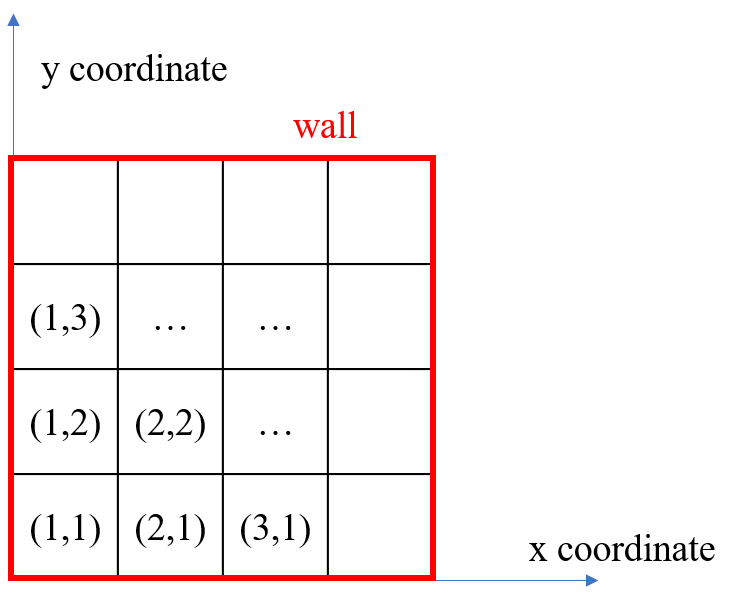
\includegraphics[width=6cm]{RandomWalkGrid.png}       
	\caption{Coordinate representation in spatial grid}
\end{figure}

The dynamics of a particle are relatively straightforward and can be described by equation \ref{eq:RandomWalkDynamics}. A particle has 5 options for its motion: moving up, right, down, left or no motion (options are depicted in figure \ref{fig:RandomWalkMotion}). Every motion has a certain probability $p$ to occur. These probabilities can be given as input and must add up to 1.

\begin{equation}
\label{eq:RandomWalkDynamics}
X_{k+1}(x,y) = X_k(x,y) +  \begin{cases}
(0,1) &\text{with probability $p\uparrow$}\\
(1,0) &\text{with probability $p\rightarrow$}\\
(0,-1) &\text{with probability $p\downarrow$}\\
(-1,0) &\text{with probability $p\leftarrow$}\\
(0,0) &\text{with probability $p\ \bullet$}
\end{cases}
\end{equation}



\begin{figure}[htb]
    \label{fig:RandomWalkMotion}
	\centering
	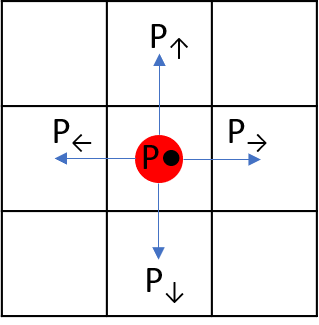
\includegraphics[width=3cm]{RandomWalkMotion.png}       
	\caption{Potential motion per time step}
\end{figure}


\paragraph{Implementation} 
At the top of the file, it is possible to set the grid size, starting position of particles, \# of particles, simulation horizon and motion direction probabilities. The script will also generate snapshots of the particle distribution at different moments in time during the simulation. By selecting the number of subplots, you can determine how many instances you would like to see. This will provide insights into how the particle distribution develops over time. \newline

Particles are simulated one at a time. The simulation runs until the time horizon $T$ is reached or the particle hits the wall. Their position is saved in a 3-dimensional array (time, x-position, y-position) at specified moments in time only; this way the amount of required memory is kept to a minimum. %You do not save the position of every particle at every time step, but you only ``count'' their positions at time steps that you are interested in. Information about individual particles gets lost, but that is fine.
\newline

Information about where particles hit the wall is included in the same arrays. This data ``circumvents'' the $n \times n$ data about the particle distribution within the grid. As a result, when we plot the full array we can see the distribution of particles in the grid at their respective location, and the distribution of particles at the wall directly ``behind'' the wall.\newline

\begin{python}
# This file will model/simulate the random motion

import numpy as np
import matplotlib.pyplot as plt
from random import *
import pylab

############## START INPUT #################

GridSizeSquare = 20 # n, will create an nxn grid
#define starting position as ratio or grid size
Pos_init = np.ceil(np.array([0.4,0.4])*GridSizeSquare)
#T is the total amount of time steps, scale with square of grid size. 0.3 is nice
T = 0.3*np.power(GridSizeSquare, 2)
n_particles = 10000 # #particles. 10000+ recommended
# define the # of subplots for intermediate time snap shots
subplot_row = 2             
subplot_column = 2
#defines the drift probabilities: ([up,right,down,left,0]) 
motion_prob = np.array([0.2,0.2,0.2,0.2,0.2])

############## END INPUT #################

#only look at square grids, but this could be changed:
x_grid = GridSizeSquare
y_grid = GridSizeSquare
n_subplot = subplot_row*subplot_column
Plot_interval = np.floor((T-1)/(n_subplot-1))
#This determines when you take snapshots of the process, every "Plot_interval" time steps

# now define the probabilities of the random walk
# notation of motion ([up,right,down,left,no motion])
# I normalized in case probabilities do not add up to 1...
motion_prob = motion_prob/np.sum(motion_prob)
# define the change in coordinates of every motion:
motion_xy = np.array([[0,1],[1,0],[0,-1],[-1,0],[0,0],])
motion_prob_percentile = np.cumsum(motion_prob)
# this is used later to draw from with randomizer

# make an empty data grid from where you are going to count the amount occurrences and hits against the wall
Data = np.zeros((x_grid+2,y_grid+2)) # "+2" for wall data
Data_resized = np.zeros((Data.shape[0]+1,Data.shape[1]+1))
# This for plotting purposes, I need to add an extra row an column for some reason
# Now create a new empty data set for the intermediate plots:
Data_TimeVarying = np.zeros((n_subplot,Data_resized.shape[0],Data_resized.shape[1]))

# construct some arrays for plotting later on:
xx, yy = pylab.meshgrid(
    pylab.linspace(-1,x_grid+1,x_grid+3),
    pylab.linspace(-1,y_grid+1,y_grid+3))

# Here, start loop over all the particles after each other:
for i in range(1, n_particles+1):
    # Initialize simulation
    t = 0
    HitWall = False
    Pos = Pos_init
    Subplot = 1
    
    # start simulation
    while t < T and not HitWall:
                
         # Now continue with the motion simulation
        MotionRandom = random()
        IndexMotion = np.argmax(motion_prob_percentile>MotionRandom)
        Pos = Pos + motion_xy[IndexMotion,:] #this works
        
        # Now check for hitting the wall
        if Pos[0] == 0 or Pos[1] == 0 or Pos[0] == x_grid+1 or Pos[1] == y_grid+1:
            if Subplot <= n_subplot:             
                Data_TimeVarying[Subplot-1,Pos[0],Pos[1]] = Data_TimeVarying[Subplot-1,Pos[0],Pos[1]]+1
            HitWall = True

        # Now record the position for time dependent plotting purposes
        if t % Plot_interval == 0 and Subplot <= n_subplot and not(HitWall):   #so create a subplot every Plot_interval time steps
            Data_TimeVarying[Subplot-1,Pos[0],Pos[1]] = Data_TimeVarying[Subplot-1,Pos[0],Pos[1]]+1
            Subplot = Subplot+1        
        
        t = t+1
    
    
    #This was basically the whole simulation, now save the results
    Data[Pos[0],Pos[1]] = Data[Pos[0],Pos[1]] + 1
    # I need to give resize Data with an extra row and column, since pcolor doesn't plot the full range of the matrix...
    Data_resized[:-1,:-1] = Data       


# Now I need to do some post-processing of the intermediate measurements.
# I need to add the particles that hit the wall in earlier time steps to the 
# later plots, so the total amount of particles is always n  
Data_TimeVarying_Corrected = np.cumsum(Data_TimeVarying,axis=0)
Data_TimeVarying_Corrected[:,1:x_grid+1,1:y_grid+1] = Data_TimeVarying[:,1:x_grid+1,1:y_grid+1]


# This loop creates subplots at several time instances
plt.figure()
for j in range(1, n_subplot+1):
    #Now visualize the outcomes
    pylab.subplot(subplot_row, subplot_column, j)
    pylab.pcolor(xx,yy,np.transpose(Data_TimeVarying_Corrected[j-1,:,:]))
    TitleString = 'Distribution at t = ' + str((j-1)*Plot_interval+1)
    pylab.title(TitleString)
    # and a color bar to show the correspondence between function value and color
    pylab.colorbar()
    pylab.hold(True)
    pylab.plot([0, x_grid],[0, 0], 'r',[0, x_grid],[y_grid, y_grid], 'r',[0, 0],[0, y_grid], 'r',[x_grid, x_grid],[0, y_grid], 'r')
    pylab.plot(Pos_init[0]-0.5,Pos_init[1]-0.5,'ro')

pylab.show()

# This plot shows the final distribution, including distribution along the walls
plt.figure()
pylab.pcolor(xx,yy,np.transpose(Data_resized))
pylab.title('Final distribution at t = %d, including hitting walls' %T)
# and a color bar to show the correspondence between function value and color
pylab.colorbar()
pylab.hold(True)
pylab.plot([0, x_grid],[0, 0], 'r',[0, x_grid],[y_grid, y_grid], 'r',[0, 0],[0, y_grid], 'r',[x_grid, x_grid],[0, y_grid], 'r')
pylab.plot(Pos_init[0]-0.5,Pos_init[1]-0.5,'ro')
pylab.show
\end{python}



\paragraph{Results}
In this section we included two simulation for both a $10x10$ grid and a $20 \times 20$ grid, with a different simulation time horizon $T$. Both simulations use 10,000 particles and have a motion probability of $0.2$ in all directions. \newline

It is clearly visible how the particles spread out over time and make their way to the walls over time. The more particles that are simulated per grid resolution, the smoother the distribution becomes. You can clearly see that 10,000 particles simulated lead to a clean distribution in the smaller plot of figure \ref{fig:RandomWalk10}, while the larger plot of \ref{fig:RandomWalk20} shows a more grainy distribution.

\begin{figure}[htb]
    \label{fig:RandomWalk10}
	\centering
	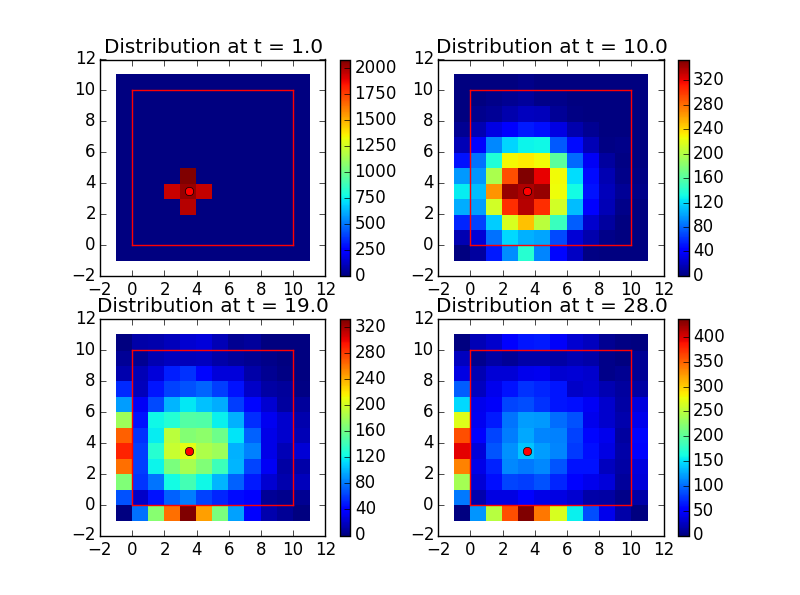
\includegraphics[width=14cm]{figure10x10.png}       
	\caption{Particle distribution for $10 \times 10$ grid at different time steps}
\end{figure}

\begin{figure}[htb]
    \label{fig:RandomWalk20}
	\centering
	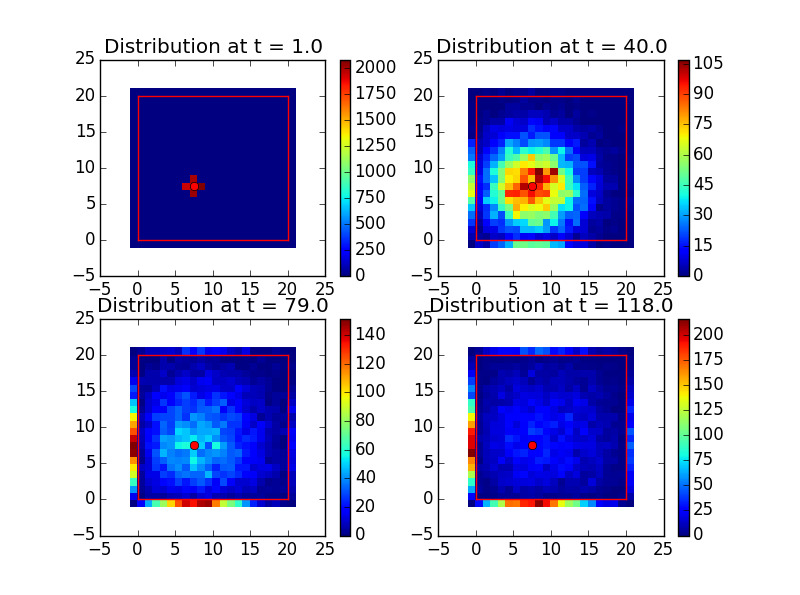
\includegraphics[width=14cm]{figure20x20.png}       
	\caption{Particle distribution for $20 \times 20$ grid at different time steps}
\end{figure}


 
\paragraph{Interpretation}
{\it Relate these quantities to the model and to theoretical knowledge of the course.}\newline

{\it I think this motion is described by Fick's Law in 2 dimension. The concentration on a specific point changes over time, depending on the concentration of its surroundings. Should we derive why the second derivative matters? $\phi$ is the concentration, $D$ the diffusion coefficient.}

\begin{equation}
\label{eq:FicksLaw}
\frac{d\phi}{dt} = D\nabla\phi = D \big(\frac{d^2\phi}{dx^2} + \frac{d^2\phi}{dy^2}\big)
\end{equation}


 \paragraph{Conclusion}
 \textit{What have we learned? Is everything aligned (theory and practice)? What was difficult? Provide perspectives.}
 
 The dynamics of the random walk were easy to model. The challenge in this simulation was to save the data for the intermediate time steps. Since the particles are simulated one by one for the full time horizon, we had to write some non-intuitive code to save the location of every particle at the relevant intermediate time steps. \newline
 
 From the lecture we recall that diffusion distance scales with the square root of time. Here we tried to simulate that. When doubling the grid size and taking a four times higher simulation horizon, the distribution looks similar. However, we have the idea that the scaling did not work for 100\%. At the end of the scaled simulation horizon, it seems as if the smaller grid has relatively more particles in the grid than the larger grid has. What could cause this difference?
 

\thispagestyle{empty}
%----------------------------------------------------------------------
\chapter{Control and optimization}
\label{control.chap}
%----------------------------------------------------------------------

\section{Objectives}
%----------------------------------------------------------------------
Once a system has been enough understood, there is still to do the main work: enhance it. This means most of the time optimization, and control can be seen as an online optimization (i. e. continuously making the system better). There are several control techniques as there are many optimization techniques. Since this reader aims at keeping things practical, we will not develop all possible ideas here. Instead we insist onto 2 main ideas:
\begin{enumerate}
	\item explicit a criteria to be optimized: in principle, this is rooted in the system description and what we want to do with the system. There are many ways to enhance a system, and very often the models are too complicated to have an explicit optimum (whenever they have one). But without criteria, there is even no way to know what is better (or worse).
	\item simplify the model so that the optimization (or control) problem can be solved by simple tools. As a rule, it is often better to get a simple but efficient control rather than to try to compute the optimal one. This rules also holds for optimization: the best is the enemy of the good; well enough is enough in lots of practical systems.
\end{enumerate}

Therefore some tools for PDE are applied in the next sections as well as simple tools that can be applied by smartly simplifying the problem.

\section{Tools and examples}

\subsection{Kalman filter}
% ***********************************************************************************
% Pure LaTeX part to be inserted in a document (be careful of depencies of packages & commands
% Prepared by XXX and YYY under the supervision of Arnaud de La Fortelle
% Fall 2017
% 2D wave propagation subsection of the modeling part
% ***********************************************************************************


\paragraph{Control model}

We consider here the simplest model for which a Kalman filter can really bring an added value: a linear, Gaussian and real (i.e. 1D) model:
\begin{eqnarray}
\label{kalman-dynamics.eq1}
x_{k+1} &=& A x_k + B u_k + v_k\\
\label{kalman-dynamics.eq2}
y_k &=& C x_k + w_k
\end{eqnarray}
where $X=(x_k)$ is the state of the system (typically a distance to a prescribed value, in whatever unit), $U=(u_k)$ is the control, $Y=(y_k)$ is the measurement. $V=(v_k)$ (resp. $W=(w_k)$) is a Gaussian noise: the $v_k$ (resp. $w_k$)are independent and identically distributed random variables with 0 mean and variance $Q$ (resp. $R$). The initial state $x_0$ is also a centered random variable with variance $\bar{P}_O$. Note that these notation perfectly adapt to multidimensional systems, with matrices: see any textbook on control to get the matrix equations.

This is not specifically needed for Kalman filter, but the usual optimization criteria is quadratic:
\begin{equation}\label{kalman-cost.eq1}
	J(X,U) = \frac{1}{N}\sum_{k=0}^N \alpha u_k^2 + \beta x_k^2
\end{equation}

The Equations~(\ref{kalman-dynamics.eq1})-(\ref{kalman-dynamics.eq2}) are often written for each time step so the scaling with respect to time has to be careful. In a system with a 100 Hz time step (also refered to as control frequency), typical values are:
\begin{eqnarray*}
A &=& 1.001\\
B &=& .01\\
C &=& 1\\
Q &=& .001\\
R &=& .01
\end{eqnarray*}
We have taken $C=1$ because most of the time we try to have a measurement as close to the state as possible and if $C\neq 1$ it is possible to compensate it. $A>1$ means that the system is unstable: Figure~\ref{Kalman-free.fig} shows the divergent behavior.

\begin{figure}[htb]
	\centering
	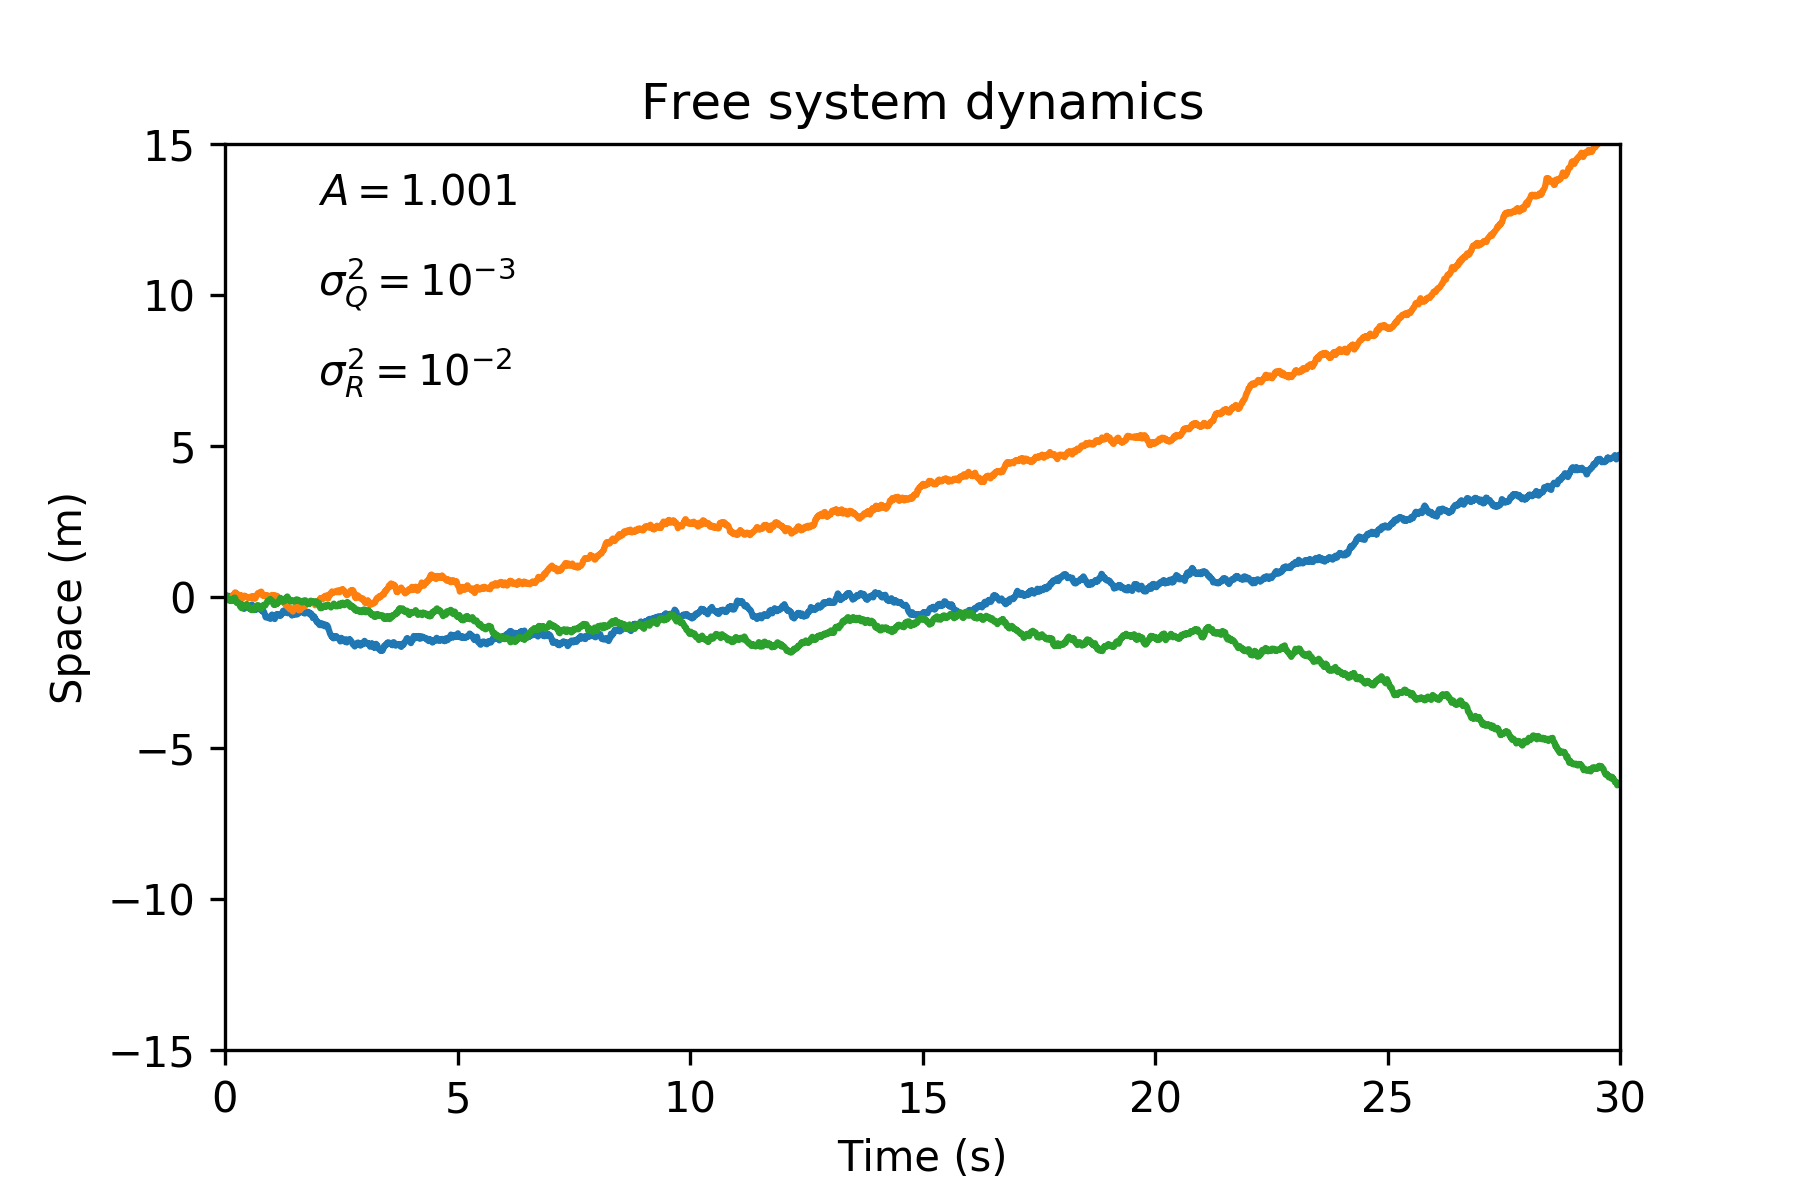
\includegraphics[width=10cm]{Kalman-free}       
	\caption{The free system dynamics: it shows instability and the system tends to diverge exponentially. The variance $\sigma_R^2$ (resp. $\sigma_Q^2$ ) is denoted by $R$ (resp. $Q$) in the system model.}
	\label{Kalman-free.fig}
\end{figure}

\paragraph{A naive control}
Now, we would like to stabilize the state of the system as close to zero as possible, and if possible at a reasonable cost. This means we can adjust the weights $\alpha$ and $\beta$ in the cost function~(\ref{kalman-cost.eq1}). Or simpler measure the 2 partial cost functions
\begin{eqnarray}
\label{kalman-costX.eq}
J_1(X) &=& \frac{1}{N}\sum_{k=0}^N  x_k^2\\
\label{kalman-costU.eq}
J_2(U) &=& \frac{1}{N}\sum_{k=0}^N u_k^2
\end{eqnarray}

Now, we introduce the simplest possible control: a proportional control with gain $K$ defined by:
\begin{equation}
\label{kalman-Pcontrol.eq}
	u_k = -K y_k
\end{equation}

Since we have "unit" parameters, let's start with a unit gain $K=1$. This indeed stabilizes the system as we see in Figure~\ref{Kalman-control-Gain1.fig}.

\begin{figure}[htb]
	\centering
	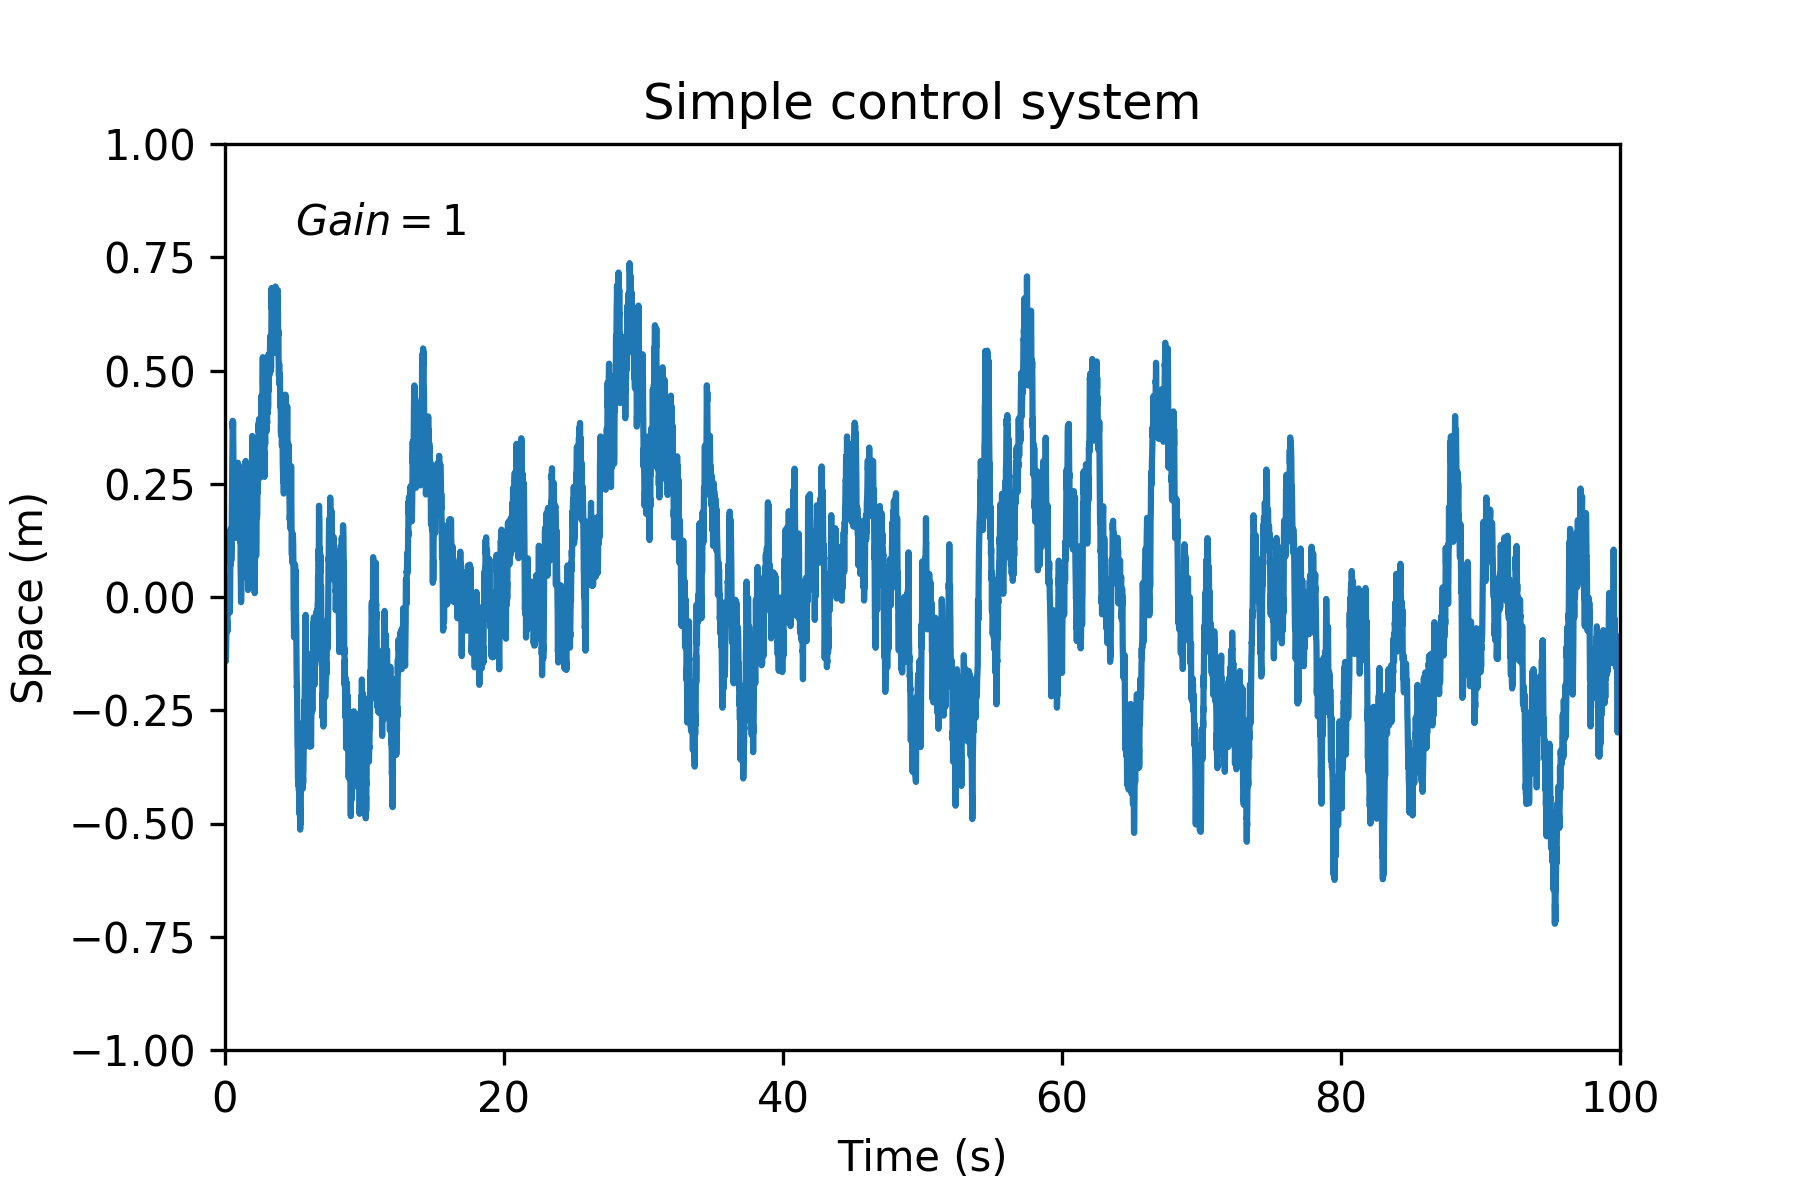
\includegraphics[width=10cm]{Kalman-control-Gain1}       
	\caption{The same system as in Figure~\ref{Kalman-free.fig} with the proportional control as defined by Equation~(\ref{kalman-Pcontrol.eq}) with gain $K=1$. The system is indeed stable with empirical costs $J_1=0.06$ and  $J_2=0.07$.}
	\label{Kalman-control-Gain1.fig}
\end{figure}

Now, if we try to maximize the precision (at all cost), we can try to compensate the term $A x_k$ in Equation~(\ref{kalman-dynamics.eq1}) by the term $B u_k = -BK Y_k = -(BKC) x_k -BK w_k$. Since we have no control onto the noise, and since this noise is centered, let's take $A = BKC$, i.e. in our case $K = A/BC = 100.1$. This lead to the result of Figure~\ref{Kalman-control-Gain100.fig}. What is impressive is not so much the increase in precision, $J_1$ is divided by about 5, that the explosion of the control cost $J_2$, multiplied by about 3,000.

\begin{figure}[htb]
	\centering
	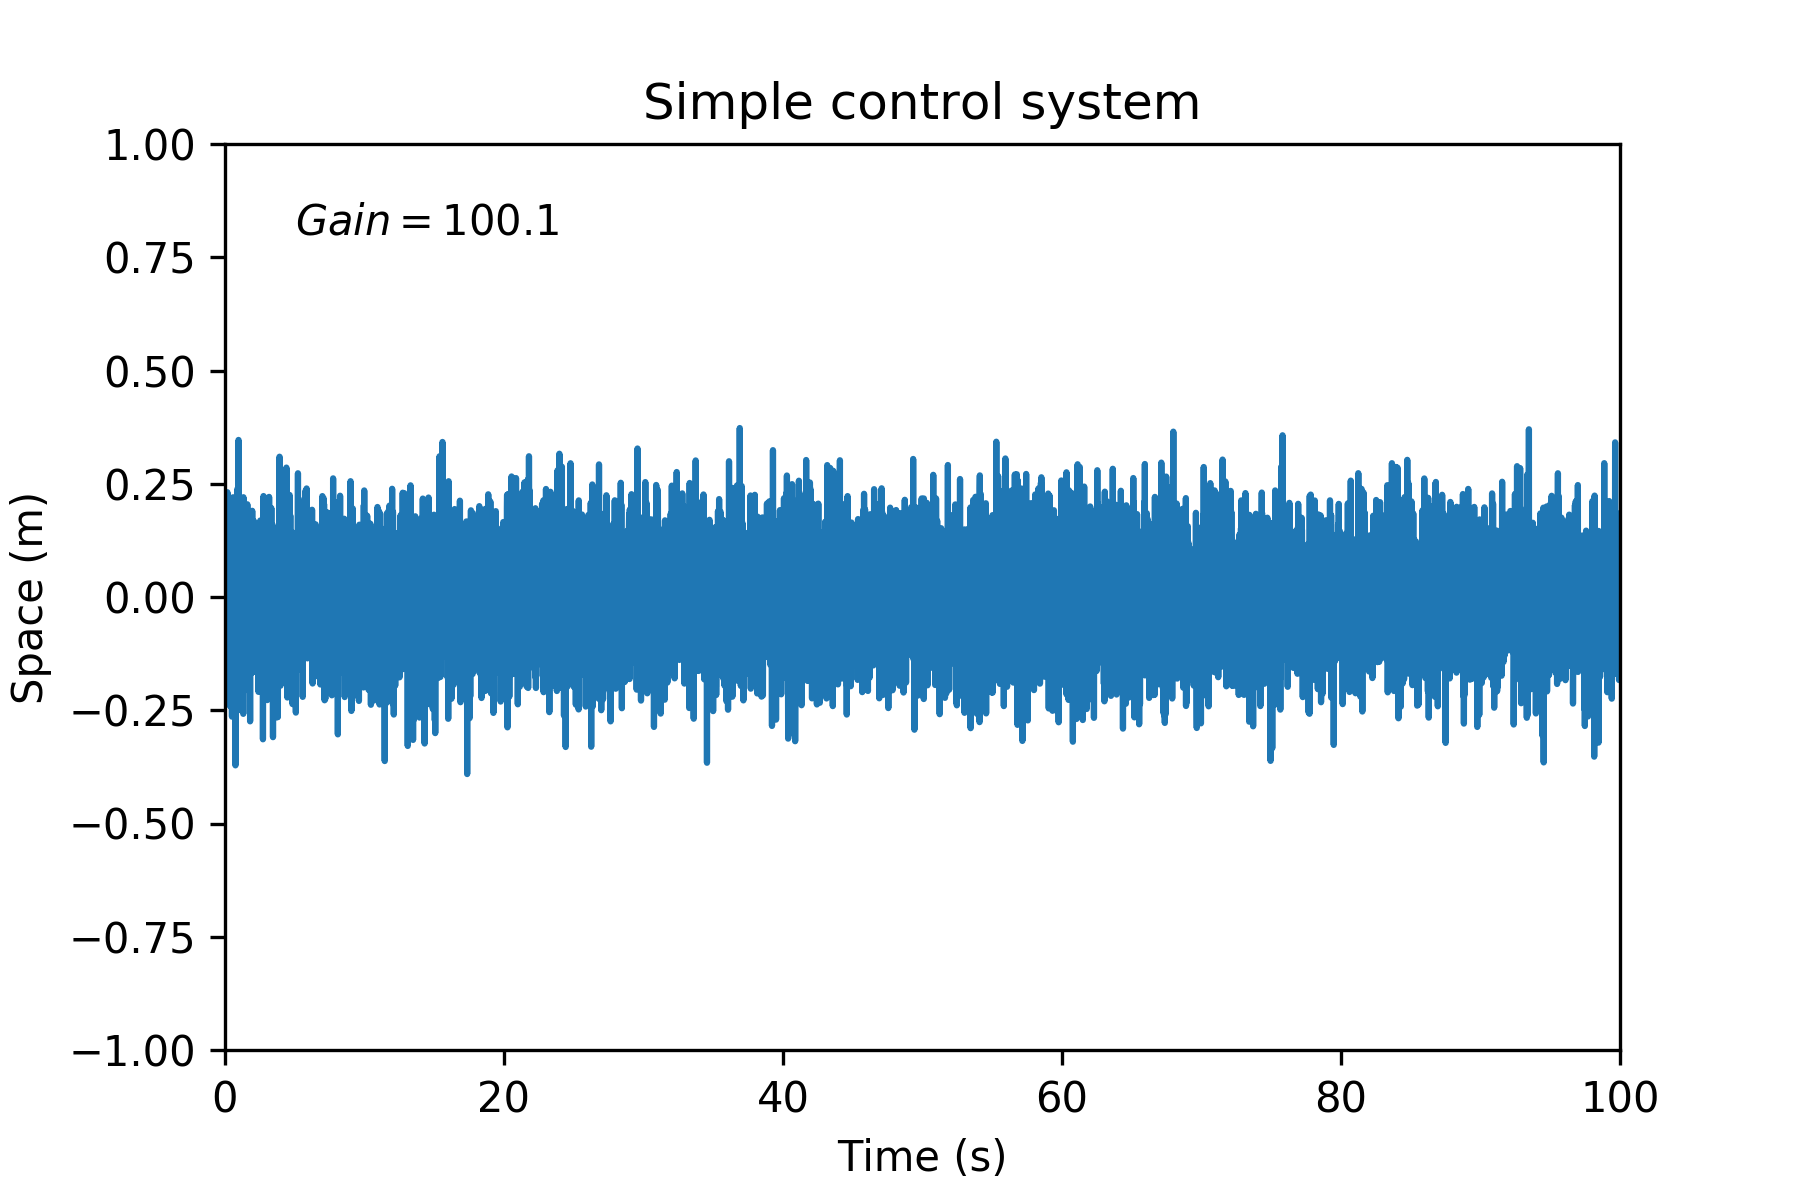
\includegraphics[width=10cm]{Kalman-control-Gain100}       
	\caption{The same system as in Figure~\ref{Kalman-control-Gain1.fig} with $K=100.1$ in order to fully compensate $A$. The system is very stable with empirical costs $J_1=0.011$ and  $J_2=209$.}
	\label{Kalman-control-Gain100.fig}
\end{figure}

In order to learn more about the trade-off between precision and control cost, one can test intermediary gains, and for $K=10$, we get the Figure~\ref{Kalman-control-Gain10.fig}. There we have a surprise: the precision is better than with our naively optimal gain $K=100.1$, not to speak of the decrease of the control cost. There are now 2 paths for us: either --- pragmatically --- adjust the gain to get the best control, or --- analytically --- try to understand what was wrong. Indeed, this numerical experiment clearly shows we are missing an important idea. And the idea we are missing is the following: we can have much better estimates of $x_k$ than $y_k$ (even after compensating some multiples in the $C$ coefficient. What we do with the heavy gain $K=100.1$ is simply to add noise. And if we go even further (e.g. $K=200$), the system becomes unstable.

\begin{figure}[htb]
	\centering
	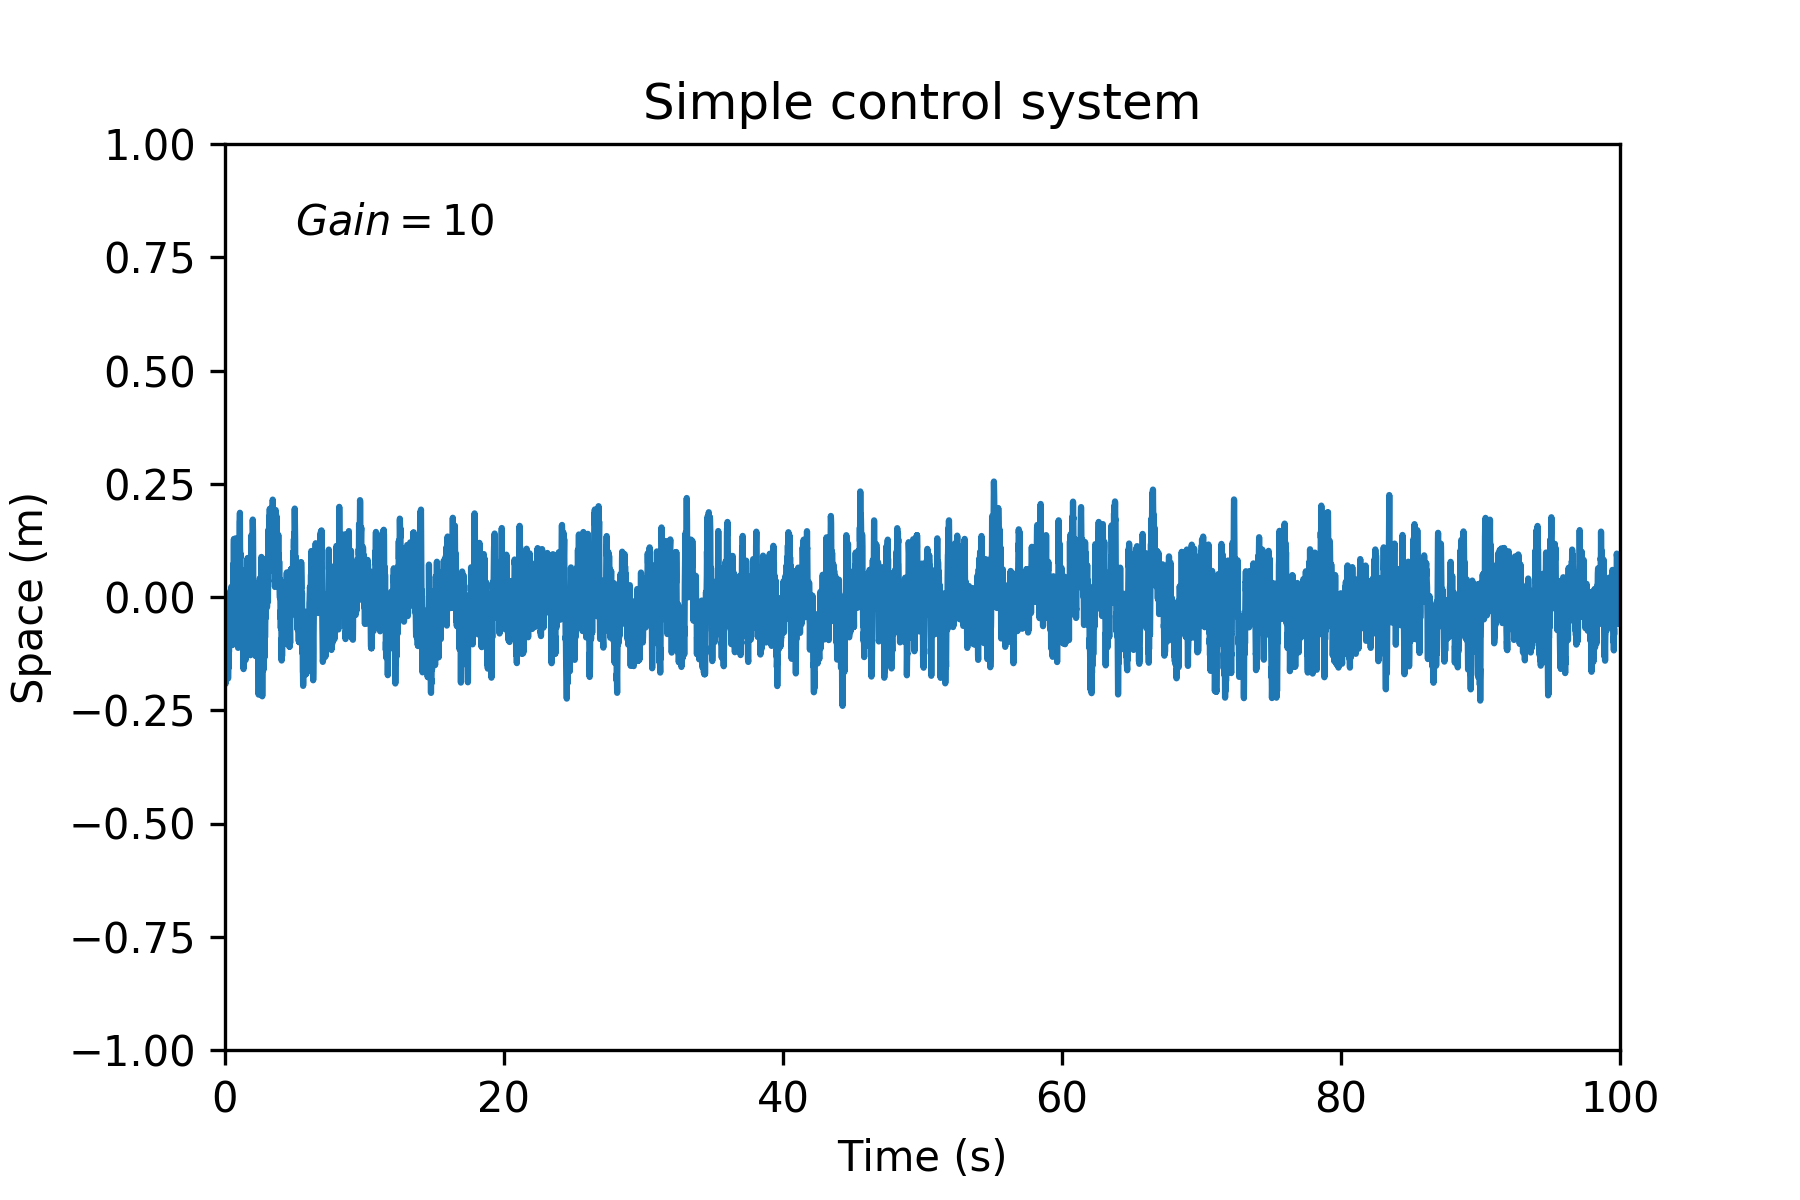
\includegraphics[width=10cm]{Kalman-control-Gain10}       
	\caption{The same system as in Figure~\ref{Kalman-control-Gain1.fig} with $K=10$. The empirical costs are $J_1=5.8\ 10^{-3}$ and  $J_2=1.59$.}
	\label{Kalman-control-Gain10.fig}
\end{figure}

\paragraph{The Kalman filter}
Now, we introduce the equations of the Kalman filter, which we know are optimal to estimate $x_k$.
\begin{eqnarray}
\label{kalman-filter.eq1}
\hat{x}_0 &=& 0\\
\label{kalman-filter.eq2}
P_0 &=& \bar{P}_0\\
\label{kalman-filter.eq3}
\hat{x}^-_{k+1} &=& A \hat{x}_k + B u_k\\
\label{kalman-filter.eq4}
P^-_{k+1} &=& A P_k A + Q\\
\label{kalman-filter.eq5}
\hat{x}_{k+1} &=& \hat{x}^-_{k+1} + L_{k+1}\left(y_{k+1}-C\hat{x}^-_{k+1}\right)\\
\label{kalman-filter.eq6}
L_{k+1} &=& P^-_{k+1}C\left(CP^-_{k+1}C+R\right)^{-1}\\
\label{kalman-filter.eq7}
P_{k+1} &=& \left(1-L_{k+1}C\right)P^-_{k+1}
\end{eqnarray}
These equations can be found in any textbook on control and are almost true as is for multidimensional states and measures. The most striking here is that the filter works whatever the control.

There is not much difference with Equation~(\ref{kalman-Pcontrol.eq}) in our control model, except that we take the best estimate:
\begin{equation}
\label{kalman-Pcontrol.eq2}
	u_k = -K \hat{x}_k
\end{equation}

This leads to the result of Figure~\ref{Kalman-TrueControl-Gain100.fig}. The precision is better than our previous best control (that was obtained for a lower gain) and the control cost is much lower than the control with same gain but based on Equation~(\ref{kalman-Pcontrol.eq}). Empirically, one sees that this gain is the optimal value in term of precision. As we are curious, we also vary the gain and we get the following results: for $K=10$, $J_1=8\ 10^{-3}$ and  $J_2=0.53$; for $K=1$, $J_1=0.072$ and  $J_2=0.069$. So we see that for lower gains (and this is much closer to realistic values), the precision is not much improved and the control cost improvement is noticeable mainly for high gains. Again, this certainly means we are missing some concepts. And here what we are missing is the notion of a better feedback control: the proportional control is too simple to be optimal. We could try a PID (Proportional-Integral-Derivative) or other controls (e.g. with pole placement), but in any case we learned that a Kalman filter allow to reduce the noise in the estimation of the state $x_k$.


\begin{figure}[htb]
	\centering
	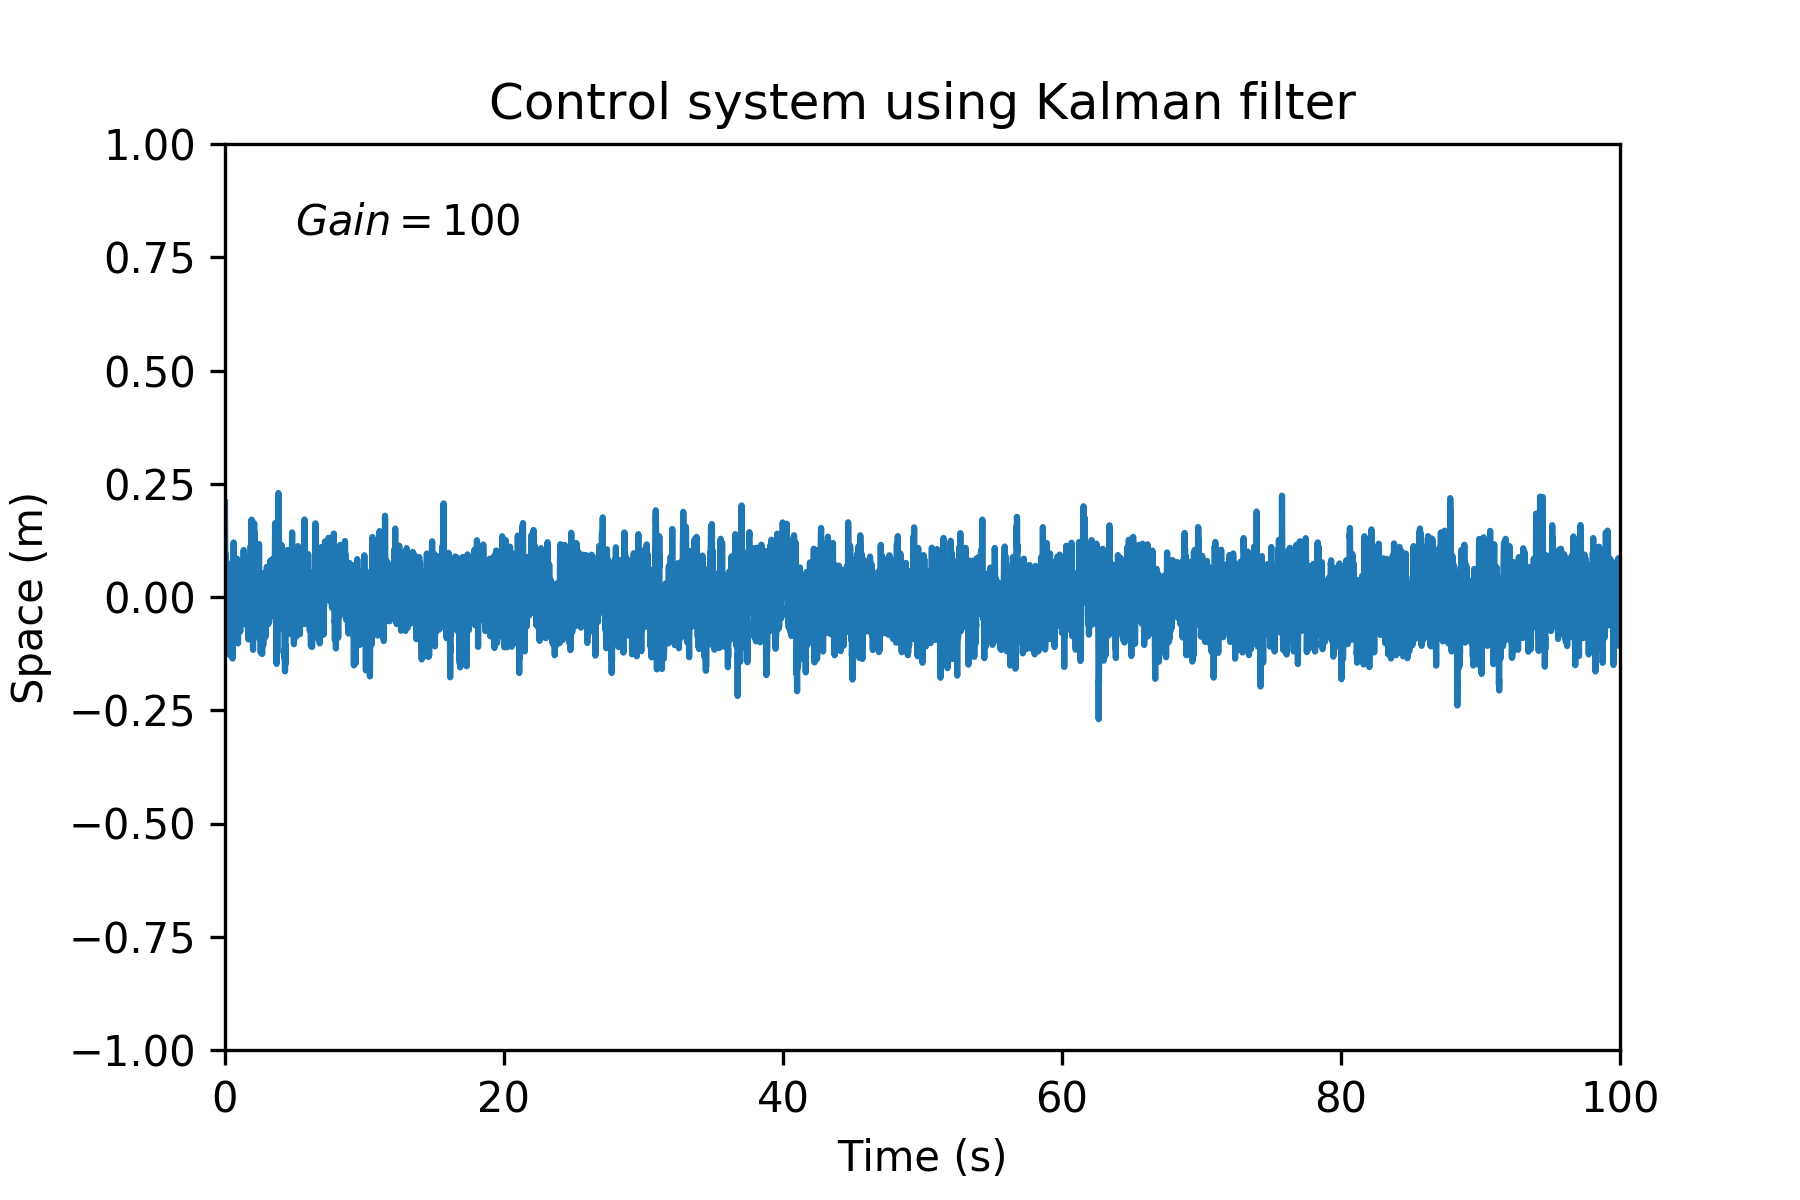
\includegraphics[width=10cm]{Kalman-TrueControl-Gain100}       
	\caption{The system with a proportional control based on Kalman filter with $K=100.1$. The empirical costs are $J_1=3.77\ 10^{-3}$ and  $J_2=10.2$.}
	\label{Kalman-TrueControl-Gain100.fig}
\end{figure}

In conclusion, note that what we learned practically about estimates, noise reduction and control are very general concepts that can be adapted to many situations, including PDEs. However, it generally requires some know-how to apply these notions.

\subsection{PID control}

\subsection{Adjoint optimization}




\end{document}



